\section{Evaluation}

The resulting thickness values for each subject were averaged within each
of the 32 labels subsequent to normalization of thickness values by the
ratio of the template volume to the individual subject volume.
Normalized cortical thickness plots (age vs. thickness) are given in Figs.
\ref{fig:nirep1}--\ref{fig:nirep3}.  The {\tt smooth.spline} function in the
R statistical project%
\footnote{
www.r-project.org/
}
was used to illustrate the trend of thinning over the course of aging. In 
several regions, there appears to be a trend of greater thickness in females
vs. males substantiating earlier findings \citep{luders2006a}. 

To test whether
gender produced statistically different regional curves, we compared 
the sum of squared residuals for a combined data curve versus the total sum of
squared residuals for the separate curves.  The resulting $p$-values calculated
from the $F$-statistic are given
in the first two columns of Table \ref{table:nirep_results} where we have 
highlighted significant differences ($p$ < 0.05).  Gender-based differences
are seen in 19 of the 32 total NIREP regions.

We also looked at hemispherical differences between corresponding lateral regions
separately in males and females.  For each gender cohort over each region we performed a pairwise $t$-test (two-tailed, $\alpha = 0.95$).  The resulting $p$-values are shown
in Table \ref{table:nirep_results} (male = third column, female = fourth column).  Whereas the male subset exhibits a statistically significant lateralization in
5 of the 16 hemispherical regions, the female subset exhibits significant lateralization
in all but one region.

\newcommand{\significant}[0]{\cellcolor[rgb]{1.0,1.0,0.8}}

%\begin{table*}
%\centering
%\begin{tabular*}{0.975\textwidth}{@{\extracolsep{\fill}} l r r r r}
%\toprule
%  \multicolumn{1}{c}{\bf NIREP Region} & \multicolumn{1}{c}{\bf Gender (left)} & \multicolumn{1}{c}{\bf Gender (right)} & \multicolumn{1}{c}{\bf Hemisphere (male)} & \multicolumn{1}{c}{\bf Hemisphere (female)} \\
%\midrule
%  occipital lobe & \significant 0.0023890 & \significant 0.0128945 & 0.9216289 & \significant $<$ 0.0000001 \\  
%  cingulate gyrus & \significant 0.0206928 & \significant 0.0104334 & 0.1675975 & \significant $<$ 0.0000001 \\
%  insula gyrus & 0.3333597 & 0.3125593 & \significant 0.0038117 & \significant $<$ 0.0000001 \\
%  temporal pole & \significant 0.0139895  & \significant 0.0386222 & 0.6284900 & \significant 0.0112162 \\
%  superior temporal gyrus & \significant 0.0017330  & 0.3326432 & \significant 0.0000487 & \significant $<$ 0.0000001 \\
%  infero temporal region & \significant 0.0000130  & \significant 0.0017276 & \significant 0.0155291 & \significant $<$ 0.0000001 \\
%  parahippocampal gyrus &  0.3031520 & 0.1200505 & \significant 0.0373879 & \significant 0.0000269 \\
%  frontal pole & \significant 0.0053043  & \significant 0.0023086 & 0.1013261 & \significant 0.0027359 \\
%  superior frontal gyrus & 0.1062380  & 0.3574514 & 0.1785346 & \significant $<$ 0.0000001 \\
%  middle frontal gyrus &  \significant 0.0028176 & \significant 0.0059724 & 0.4469982 & \significant $<$ 0.0000001 \\
%  inferior gyrus &  \significant 0.0066954 & 0.0646081 & 0.9574595 & \significant 0.0126513 \\
%  orbital frontal gyrus & \significant 0.0030429  & \significant 0.0030565 & 0.8377244 & \significant 0.0003661 \\
%  precentral gyrus & 0.9054343  & 0.7310364 & 0.1872209 & 0.2697259 \\
%  superior parietal lobule & \significant 0.0136819  & 0.0776790 & 0.3827855 & \significant $<$ 0.0000001 \\
%  inferior parietal lobule & \significant 0.0050896  & \significant 0.0366297 & 0.3740159 & \significant $<$ 0.0000001 \\
%  postcentral gyrus &  0.0628854 & 0.0896349 & \significant 0.0003167 & \significant $<$ 0.0000001 \\
%\bottomrule
%\end{tabular*}
%\caption{
%$p$-values derived from the IXI cortical thickness results 
%(highlighted values indicate $p < 0.05$).  Determination of statistical 
%differences in gender thickness curves (cf Figs. \ref{fig:nirep1}--\ref{fig:nirep3})
%over the age range $[20,30]$ are given in the first two columns.  Lateralization of 
%regional cortical thickness statistical differences are given in the third (male) and 
%fourth (female) columns.
%}
%\label{table:nirep_results}
%\end{table*}

\begin{table}
\centering
\begin{tabular*}{0.475\textwidth}{@{\extracolsep{\fill}} l r r}
\toprule
  \multicolumn{1}{c}{\bf NIREP Region} & \multicolumn{1}{c}{\bf Female} & \multicolumn{1}{c}{\bf Male} \\
\midrule
  occipital & \significant 1e-8 & 0.840\\  
  cingulate  & \significant 1e-4 & 0.762 \\
  insula & \significant 1e-7 & 0.064 \\
  temporal pole & \significant 0.047 & 0.573 \\
  superior temporal  & \significant 1e-32 & \significant 0.015 \\
  infero temporal & \significant 1e-31  & 0.169 \\
  parahippocampal & \significant 1e-3 & 0.101 \\
  frontal pole & \significant 0.010 & 0.056 \\
  superior frontal  & \significant 1e-18 & 0.451 \\
  middle frontal  & \significant 1e-12 & 0.693 \\
  inferior & 0.119 & 0.961 \\
  orbital frontal  & \significant 1e-4 & 0.803 \\
  precentral  & \significant 0.011 & 0.167 \\
  superior parietal  & \significant 1e-17 &  0.641 \\
  inferior parietal  & \significant 1e-17 & 0.654 \\  
  postcentral  & \significant 1e-31 & \significant 0.018 \\
\bottomrule
\end{tabular*}
\caption{
$p$-values derived from the IXI cortical thickness results 
(highlighted values indicate $p < 0.05$).  Lateralization of 
regional cortical thickness statistical differences are given in the third (male) and 
fourth (female) columns.
}
\label{table:nirep_results}
\end{table}

\begin{table*}
\centering
\begin{tabular*}{0.975\textwidth}{@{\extracolsep{\fill}} l r r r r r r }
\toprule
  \multicolumn{1}{c}{\bf NIREP Region} & 
    \multicolumn{1}{c}{\bf Female 20--40} & \multicolumn{1}{c}{\bf Male 20--40} & 
    \multicolumn{1}{c}{\bf Female 40--60} & \multicolumn{1}{c}{\bf Male 40--60} &  
     \multicolumn{1}{c}{\bf Female 60+} & \multicolumn{1}{c}{\bf Male 60+} \\
\midrule
L occipital & 1.92 $\pm$ 0.515 & 1.6 $\pm$ 0.475 & 1.75 $\pm$ 0.723 & 1.42 $\pm$ 0.598 & 1.51 $\pm$ 0.782 & 1.28 $\pm$ 0.689 \\
R occipital & 1.81 $\pm$ 0.562 & 1.55 $\pm$ 0.506 & 1.66 $\pm$ 0.742 & 1.37 $\pm$ 0.583 & 1.41 $\pm$ 0.769 & 1.23 $\pm$ 0.673 \\
L cingulate & 2.56 $\pm$ 0.749 & 2.23 $\pm$ 0.52 & 2.44 $\pm$ 0.632 & 2.16 $\pm$ 0.565 & 2.35 $\pm$ 0.675 & 2.04 $\pm$ 0.741 \\
R cingulate & 2.68 $\pm$ 0.732 & 2.31 $\pm$ 0.572 & 2.51 $\pm$ 0.641 & 2.21 $\pm$ 0.602 & 2.35 $\pm$ 0.71 & 2.06 $\pm$ 0.78 \\
L insula & 3.08 $\pm$ 0.598 & 2.79 $\pm$ 0.54 & 3.05 $\pm$ 0.781 & 2.72 $\pm$ 0.52 & 2.94 $\pm$ 0.892 & 2.6 $\pm$ 0.927 \\
R insula & 3.12 $\pm$ 0.639 & 2.87 $\pm$ 0.65 & 3.15 $\pm$ 0.738 & 2.78 $\pm$ 0.617 & 3.05 $\pm$ 0.841 & 2.77 $\pm$ 0.847 \\
L temporal pole & 3.76 $\pm$ 0.823 & 3.39 $\pm$ 0.875 & 3.56 $\pm$ 1.04 & 2.97 $\pm$ 0.907 & 2.99 $\pm$ 1.76 & 2.35 $\pm$ 1.41 \\
R temporal pole & 3.83 $\pm$ 0.939 & 3.41 $\pm$ 0.945 & 3.54 $\pm$ 1.13 & 3.01 $\pm$ 1.01 & 2.88 $\pm$ 1.78 & 2.26 $\pm$ 1.59 \\
L superior temporal & 2.27 $\pm$ 0.737 & 1.9 $\pm$ 0.518 & 1.97 $\pm$ 0.69 & 1.67 $\pm$ 0.599 & 1.6 $\pm$ 0.853 & 1.23 $\pm$ 0.744 \\
R superior temporal & 2.06 $\pm$ 0.598 & 1.81 $\pm$ 0.51 & 1.78 $\pm$ 0.704 & 1.53 $\pm$ 0.56 & 1.46 $\pm$ 0.839 & 1.14 $\pm$ 0.728 \\
L infero temporal & 3.12 $\pm$ 0.745 & 2.67 $\pm$ 0.713 & 2.94 $\pm$ 0.952 & 2.4 $\pm$ 0.758 & 2.53 $\pm$ 1.28 & 1.96 $\pm$ 1.09 \\
R infero temporal & 2.95 $\pm$ 0.721 & 2.57 $\pm$ 0.692 & 2.75 $\pm$ 0.92 & 2.31 $\pm$ 0.849 & 2.33 $\pm$ 1.27 & 1.82 $\pm$ 0.975 \\
L parahippocampal & 2.36 $\pm$ 0.455 & 2.19 $\pm$ 0.456 & 2.42 $\pm$ 0.558 & 2.1 $\pm$ 0.429 & 2.19 $\pm$ 0.687 & 1.91 $\pm$ 0.671 \\
R parahippocampal & 2.36 $\pm$ 0.499 & 2.22 $\pm$ 0.46 & 2.44 $\pm$ 0.595 & 2.14 $\pm$ 0.434 & 2.26 $\pm$ 0.69 & 2.04 $\pm$ 0.732 \\
L frontal pole & 2.98 $\pm$ 1.01 & 2.53 $\pm$ 0.685 & 2.76 $\pm$ 1.03 & 2.32 $\pm$ 0.885 & 2.52 $\pm$ 1.56 & 1.96 $\pm$ 1.4 \\
R frontal pole & 3.11 $\pm$ 0.956 & 2.55 $\pm$ 0.828 & 2.8 $\pm$ 1.22 & 2.35 $\pm$ 1.03 & 2.54 $\pm$ 1.69 & 1.98 $\pm$ 1.37 \\
L superior frontal & 2.37 $\pm$ 0.709 & 2.03 $\pm$ 0.601 & 2.11 $\pm$ 0.809 & 1.86 $\pm$ 0.748 & 1.95 $\pm$ 1.08 & 1.5 $\pm$ 1.09 \\
R superior frontal & 2.46 $\pm$ 0.746 & 2.13 $\pm$ 0.631 & 2.2 $\pm$ 0.864 & 1.94 $\pm$ 0.772 & 2.02 $\pm$ 1.07 & 1.6 $\pm$ 1.04 \\
L middle frontal & 2.51 $\pm$ 1.03 & 2.14 $\pm$ 0.85 & 2.23 $\pm$ 1.09 & 1.87 $\pm$ 0.835 & 2.05 $\pm$ 1.42 & 1.51 $\pm$ 1.25 \\
R middle frontal & 2.48 $\pm$ 1.09 & 2.06 $\pm$ 0.795 & 2.14 $\pm$ 1.14 & 1.83 $\pm$ 0.926 & 1.93 $\pm$ 1.44 & 1.43 $\pm$ 1.3 \\
L inferior & 2.23 $\pm$ 0.658 & 1.89 $\pm$ 0.529 & 1.95 $\pm$ 0.739 & 1.63 $\pm$ 0.58 & 1.61 $\pm$ 0.911 & 1.22 $\pm$ 0.834 \\
R inferior & 2.28 $\pm$ 0.658 & 1.96 $\pm$ 0.584 & 1.94 $\pm$ 0.775 & 1.67 $\pm$ 0.592 & 1.64 $\pm$ 0.916 & 1.26 $\pm$ 0.856 \\
L orbital frontal & 2.47 $\pm$ 0.568 & 2.17 $\pm$ 0.496 & 2.42 $\pm$ 0.669 & 2.08 $\pm$ 0.589 & 2.15 $\pm$ 0.895 & 1.86 $\pm$ 0.783 \\
R orbital frontal & 2.58 $\pm$ 0.677 & 2.25 $\pm$ 0.609 & 2.45 $\pm$ 0.768 & 2.09 $\pm$ 0.67 & 2.17 $\pm$ 0.951 & 1.86 $\pm$ 0.871 \\
L precentral & 1.75 $\pm$ 0.518 & 1.52 $\pm$ 0.56 & 1.42 $\pm$ 0.674 & 1.24 $\pm$ 0.574 & 1.22 $\pm$ 0.836 & 0.959 $\pm$ 0.817 \\
R precentral & 1.73 $\pm$ 0.621 & 1.49 $\pm$ 0.578 & 1.41 $\pm$ 0.706 & 1.23 $\pm$ 0.606 & 1.19 $\pm$ 0.781 & 0.93 $\pm$ 0.772 \\
L superior parietal & 1.87 $\pm$ 0.541 & 1.56 $\pm$ 0.444 & 1.69 $\pm$ 0.629 & 1.43 $\pm$ 0.5 & 1.44 $\pm$ 0.819 & 1.16 $\pm$ 0.813 \\
R superior parietal & 1.79 $\pm$ 0.447 & 1.51 $\pm$ 0.475 & 1.61 $\pm$ 0.62 & 1.37 $\pm$ 0.509 & 1.36 $\pm$ 0.791 & 1.1 $\pm$ 0.803 \\
L inferior parietal & 2.37 $\pm$ 0.661 & 1.93 $\pm$ 0.596 & 2.1 $\pm$ 0.864 & 1.75 $\pm$ 0.72 & 1.74 $\pm$ 1.17 & 1.27 $\pm$ 1.05 \\
R inferior parietal & 2.31 $\pm$ 0.737 & 1.91 $\pm$ 0.674 & 2 $\pm$ 1 & 1.68 $\pm$ 0.736 & 1.61 $\pm$ 1.13 & 1.15 $\pm$ 1.01 \\
L postcentral & 1.67 $\pm$ 0.552 & 1.43 $\pm$ 0.508 & 1.46 $\pm$ 0.543 & 1.24 $\pm$ 0.506 & 1.27 $\pm$ 0.739 & 0.998 $\pm$ 0.738 \\
R postcentral & 1.54 $\pm$ 0.506 & 1.32 $\pm$ 0.484 & 1.32 $\pm$ 0.581 & 1.13 $\pm$ 0.487 & 1.16 $\pm$ 0.681 & 0.913 $\pm$ 0.661 \\
\bottomrule
\end{tabular*}
\caption{
Normalized cortical thickness values (mean $\pm$ 95th percentile) derived from the IXI subjects for all 32 subjects.
Values were aggregated from the age ranges [20,40], [40,60], and $>60$ years.  
}
\label{table:nirep_results2}
\end{table*}


\begin{figure*}
  \centering
  \begin{tabular}{ccc}
  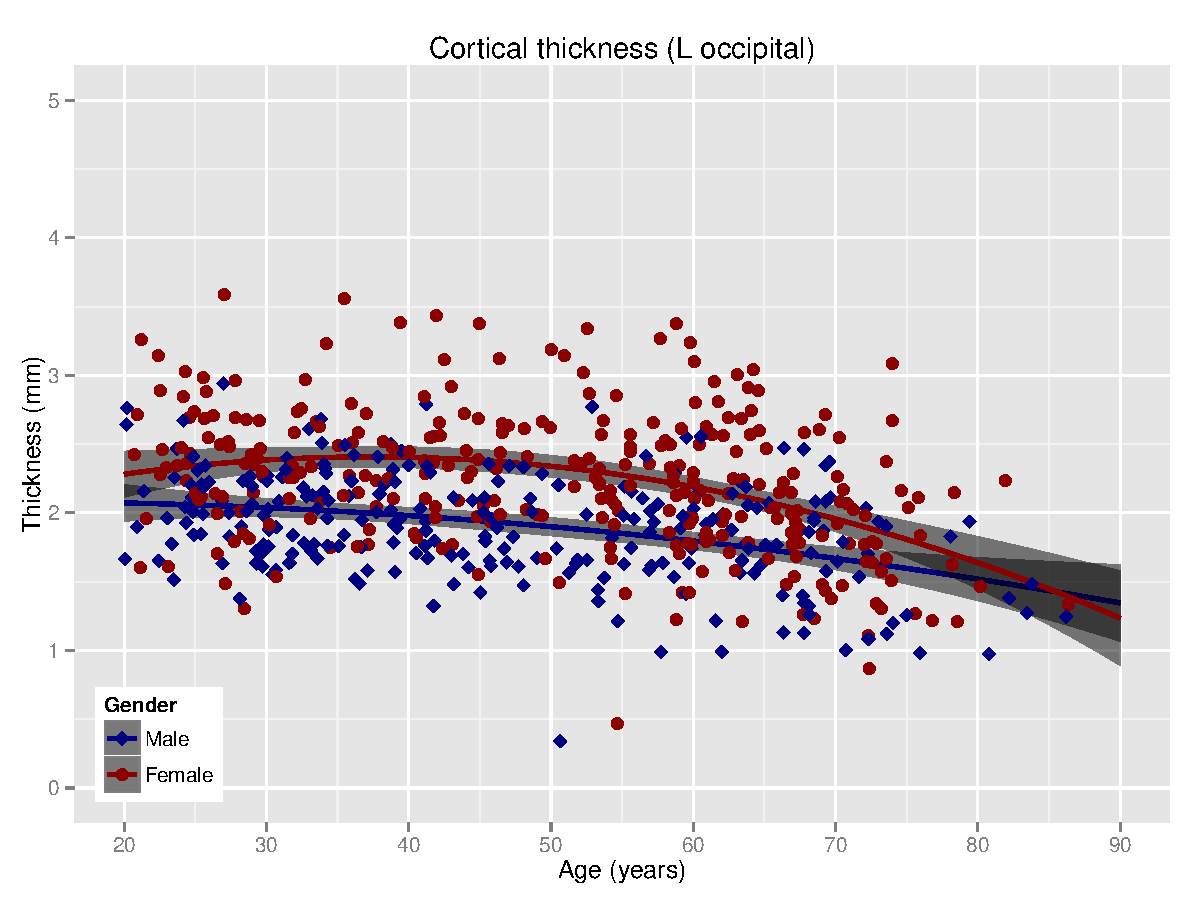
\includegraphics[width=57.5mm]{yylabel1_results.pdf} &
  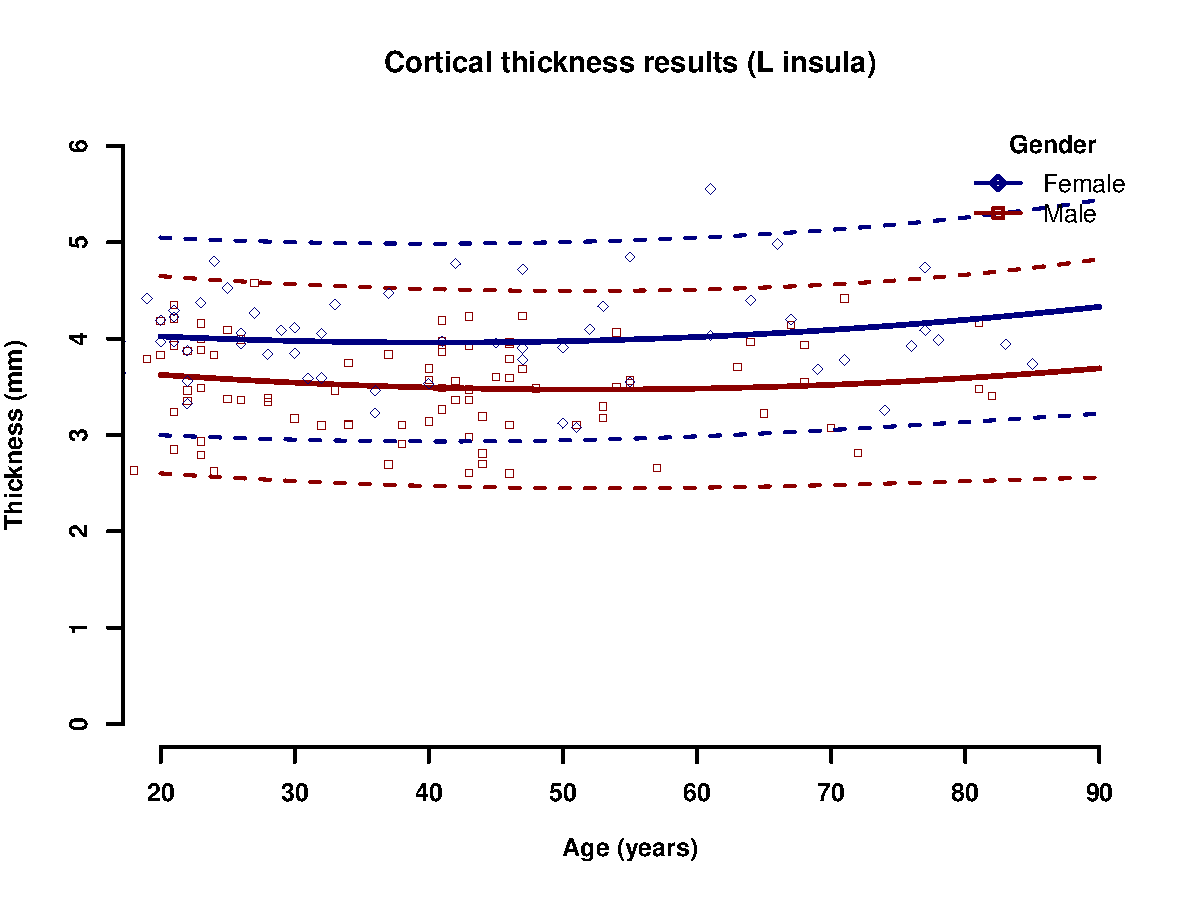
\includegraphics[width=57.5mm]{yylabel5_results.pdf} &
  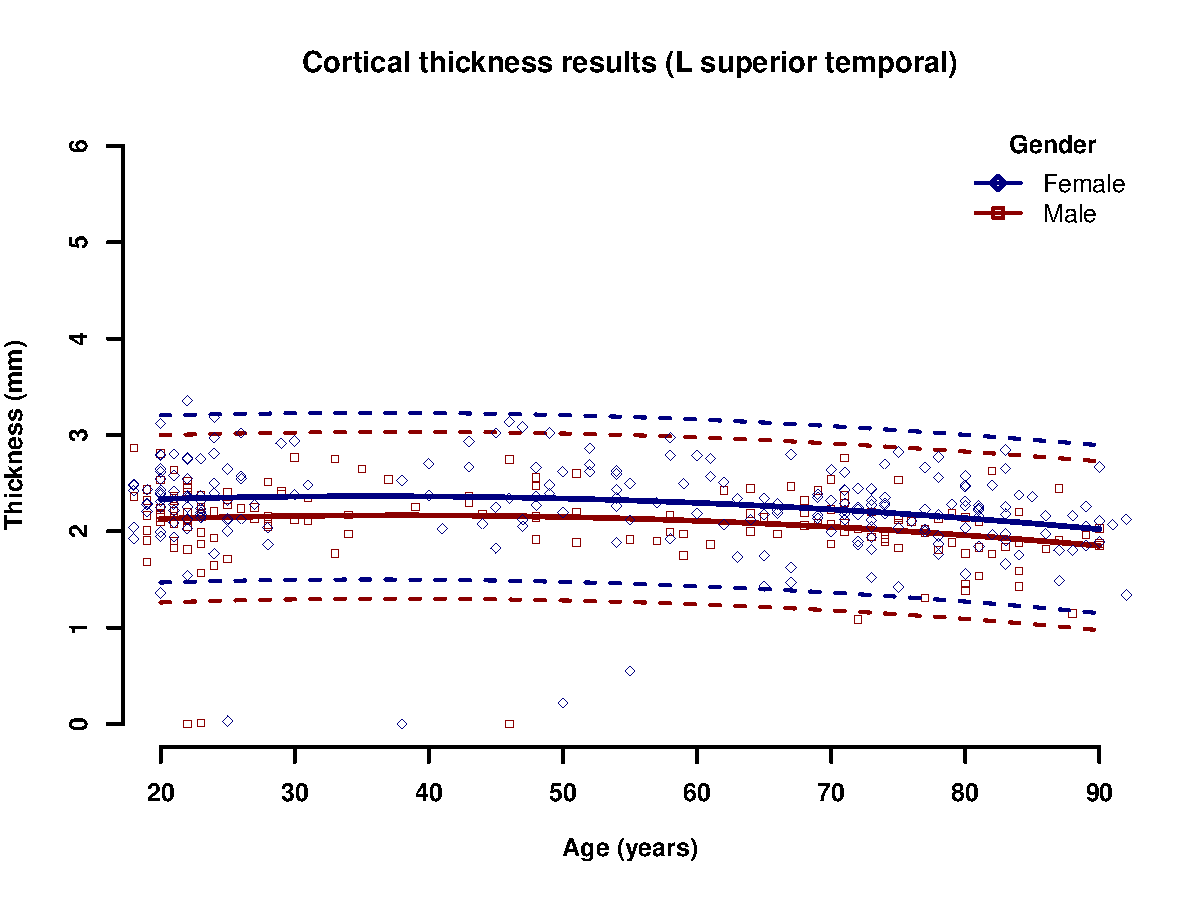
\includegraphics[width=57.5mm]{yylabel9_results.pdf} \\
  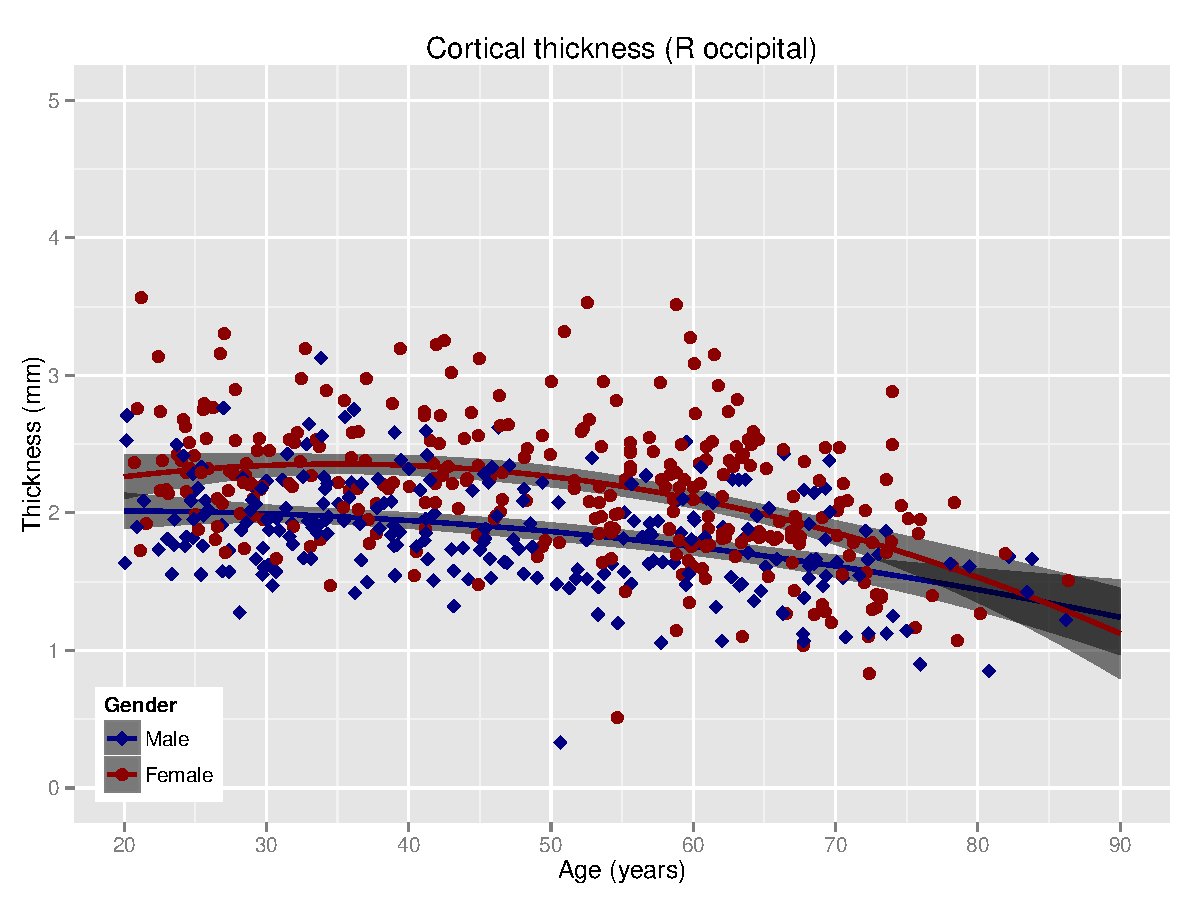
\includegraphics[width=57.5mm]{yylabel2_results.pdf} &
  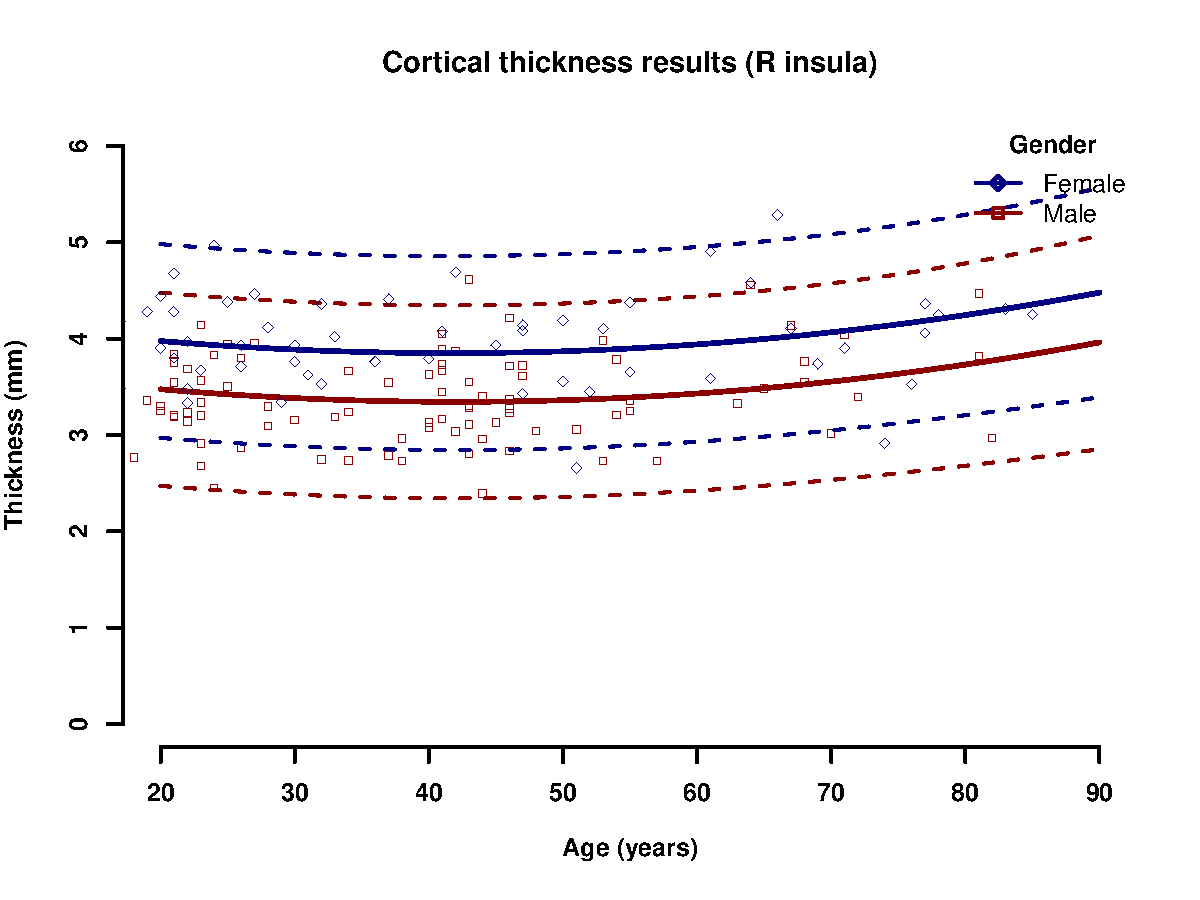
\includegraphics[width=57.5mm]{yylabel6_results.pdf} &
  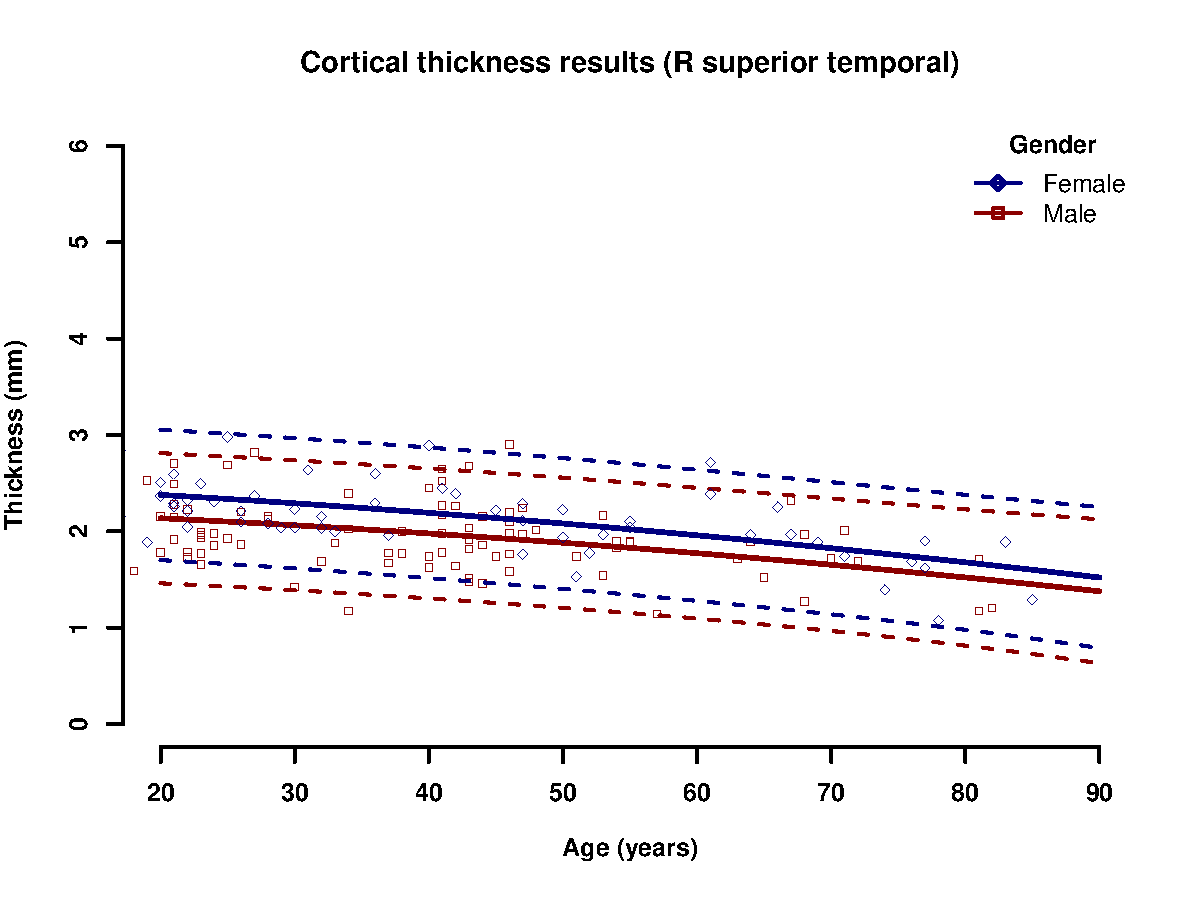
\includegraphics[width=57.5mm]{yylabel10_results.pdf} \\
  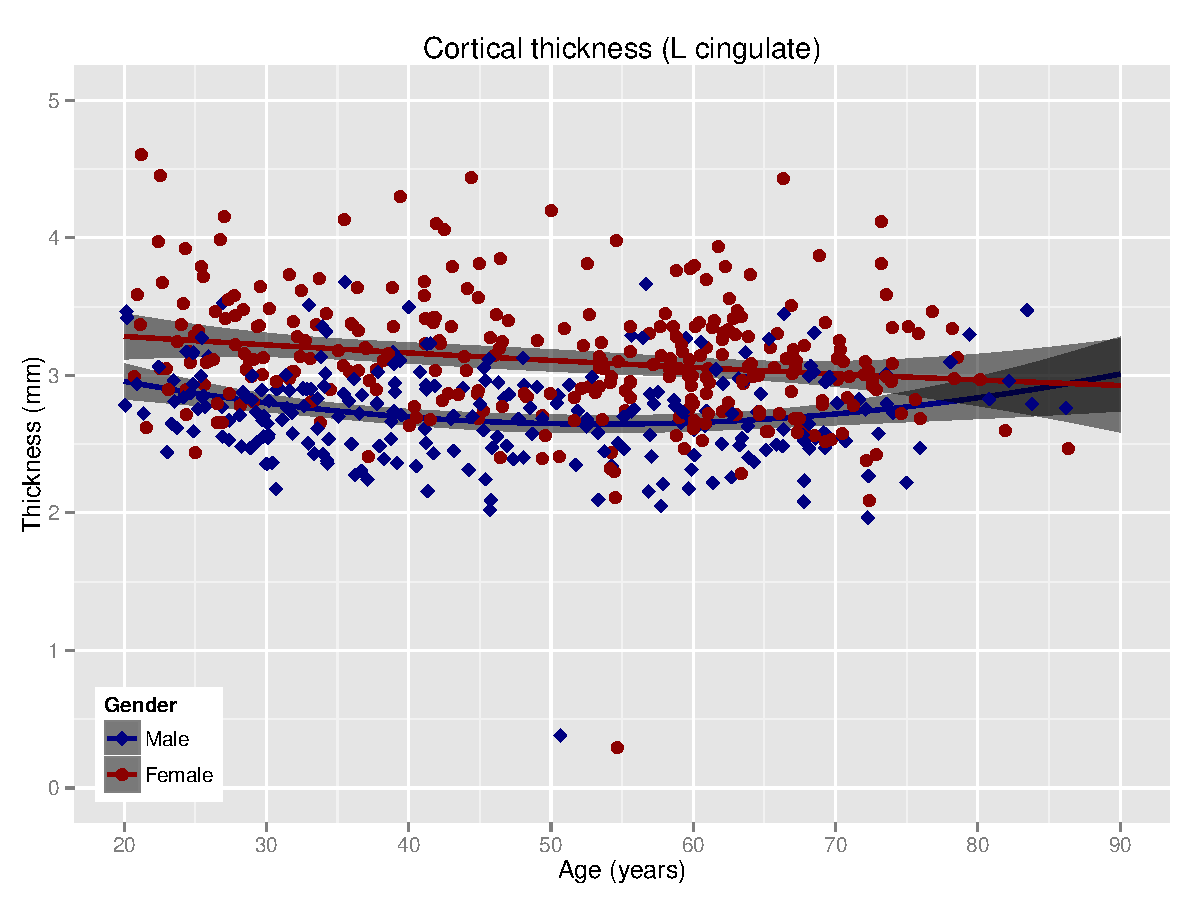
\includegraphics[width=57.5mm]{yylabel3_results.pdf} &
  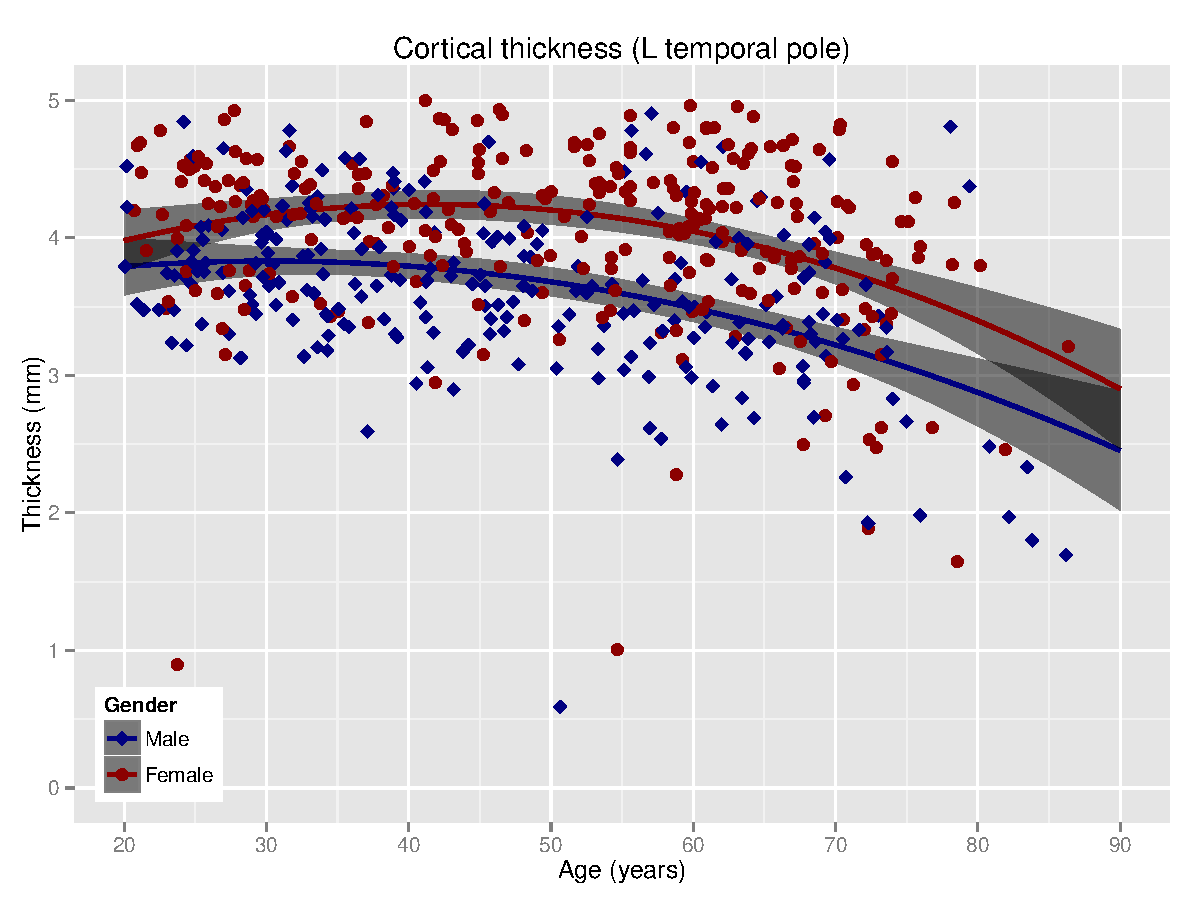
\includegraphics[width=57.5mm]{yylabel7_results.pdf} &
  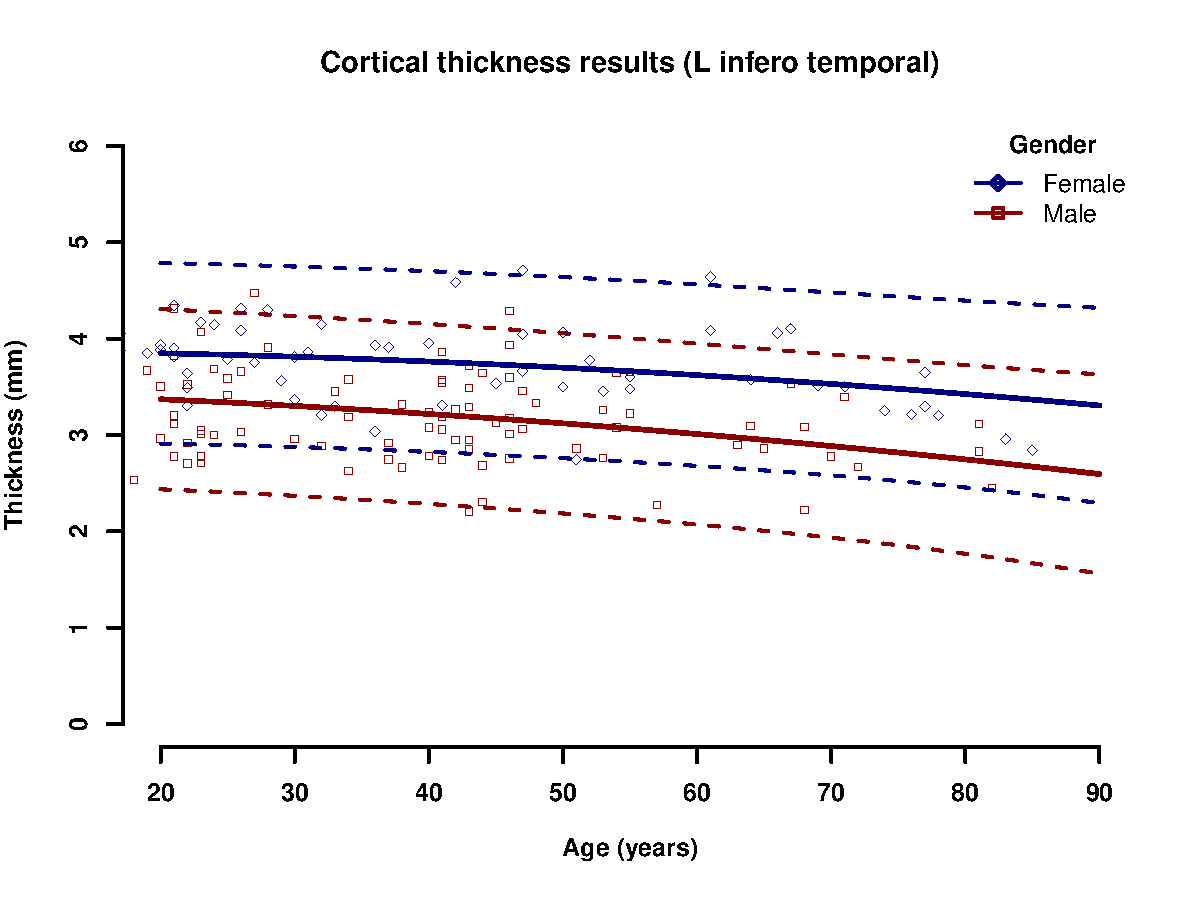
\includegraphics[width=57.5mm]{yylabel11_results.pdf} \\
  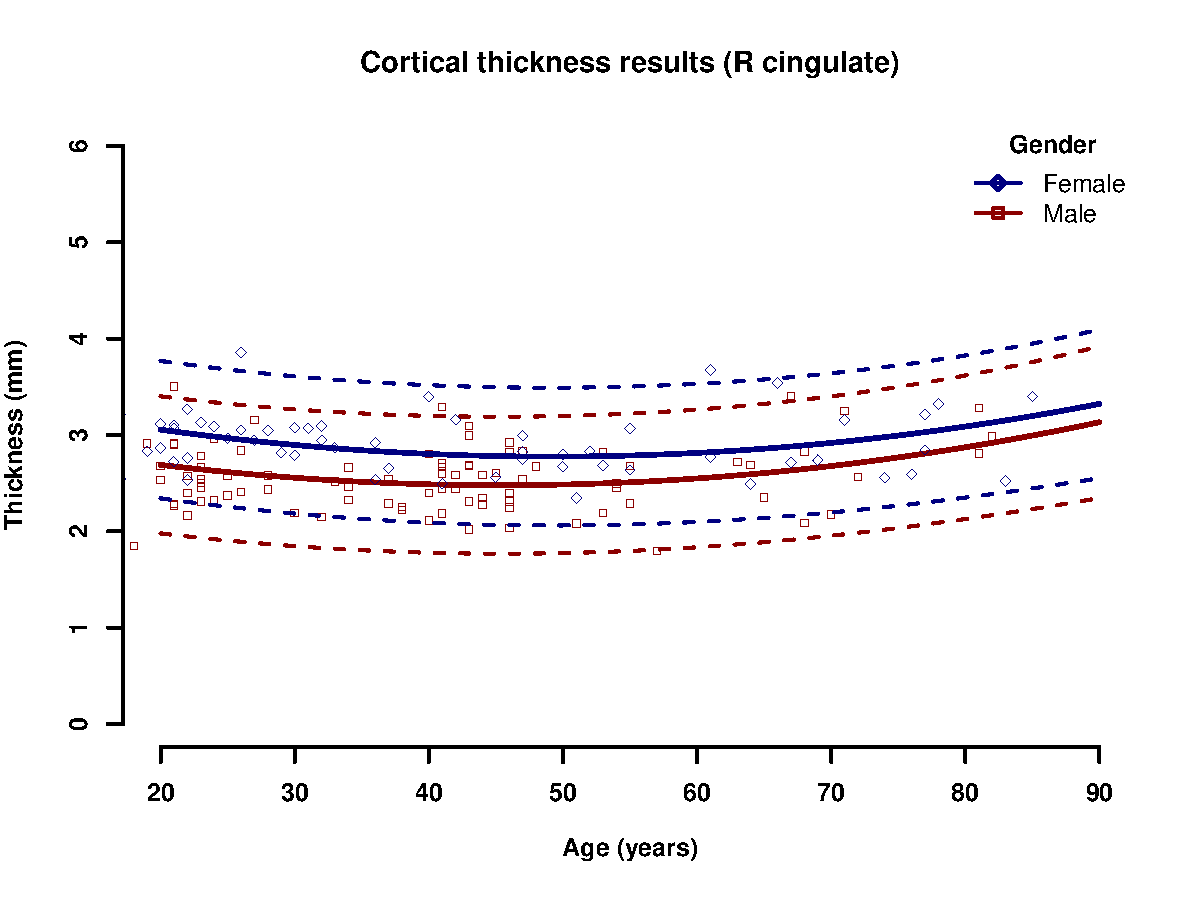
\includegraphics[width=57.5mm]{yylabel4_results.pdf} &
  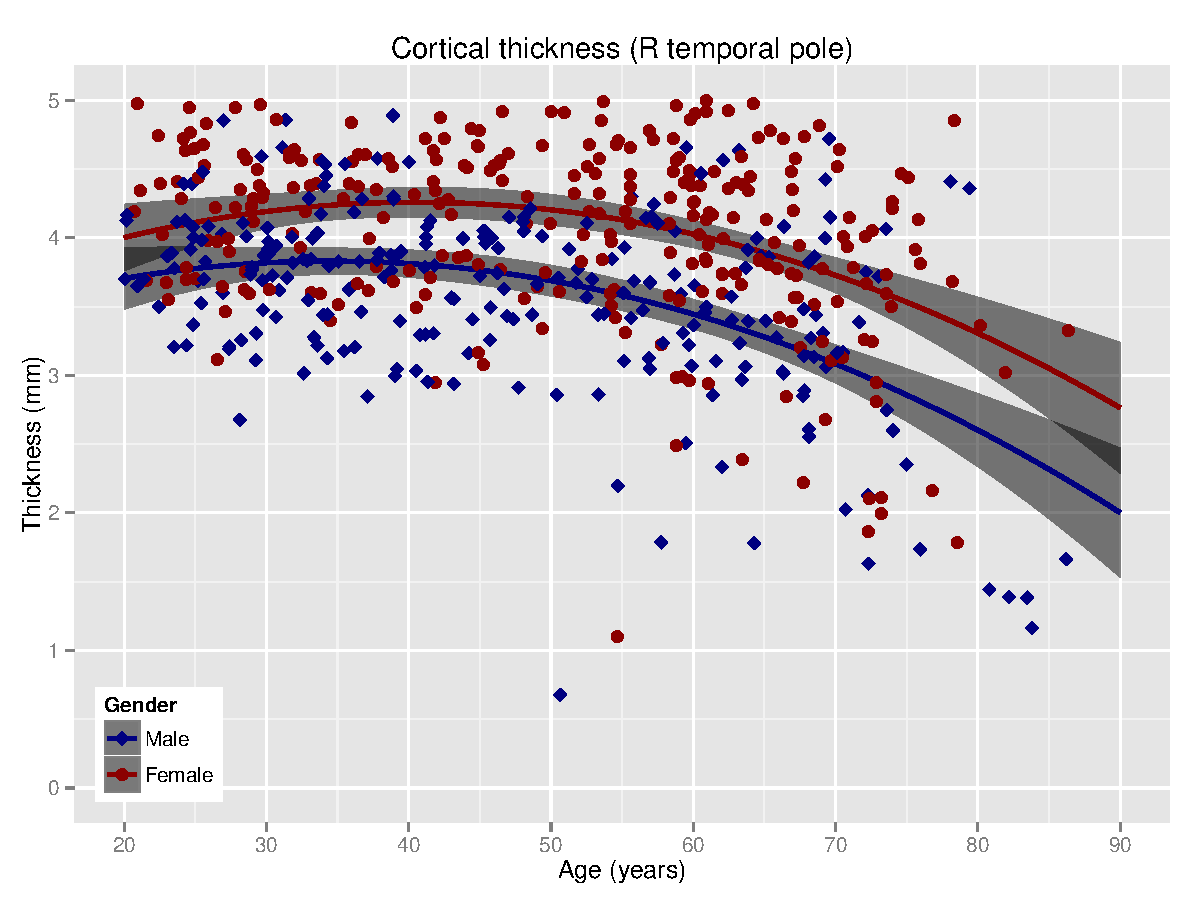
\includegraphics[width=57.5mm]{yylabel8_results.pdf} &
  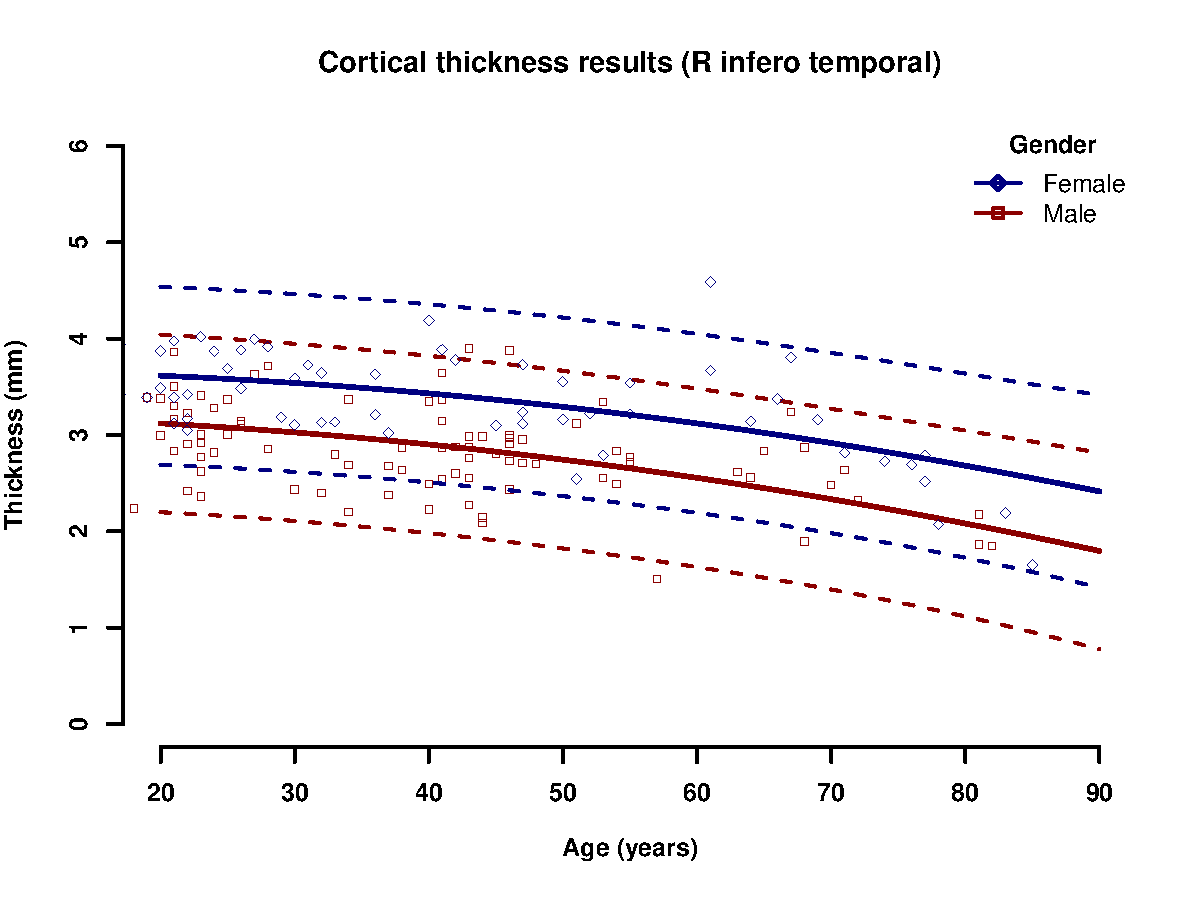
\includegraphics[width=57.5mm]{yylabel12_results.pdf} \\
  \end{tabular}
  \caption{Cortical thickness results (labels 1--12) from the IXI data set where
  each plot corresponds to one of the 32 cortical labels from the NIREP NA0 data set.  
  Thickness values have been normalized corresponding to the ratio of the individual 
  subject volume versus the total template volume.
  }
  \label{fig:nirep1}
\end{figure*}

\begin{figure*}
  \centering
  \begin{tabular}{ccc}
  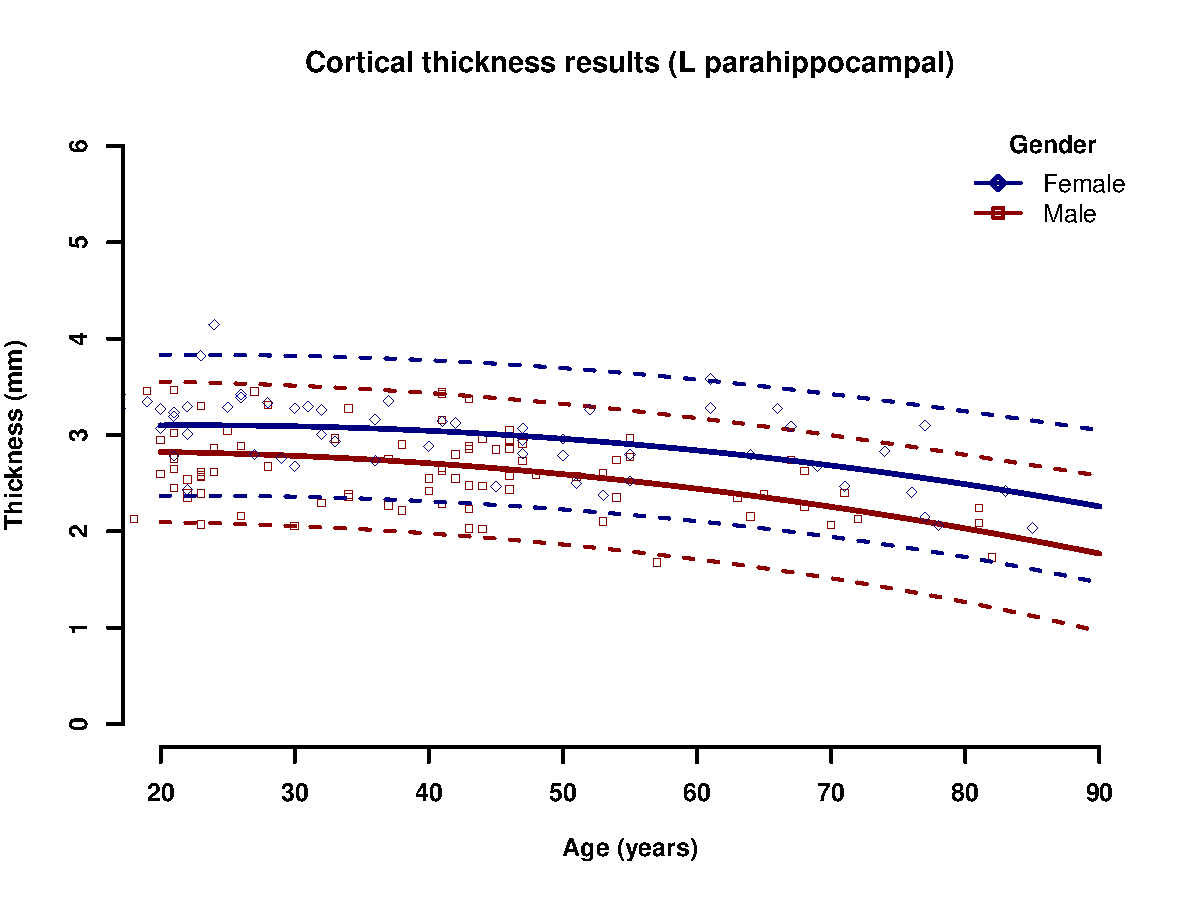
\includegraphics[width=57.5mm]{yylabel13_results.pdf} &
  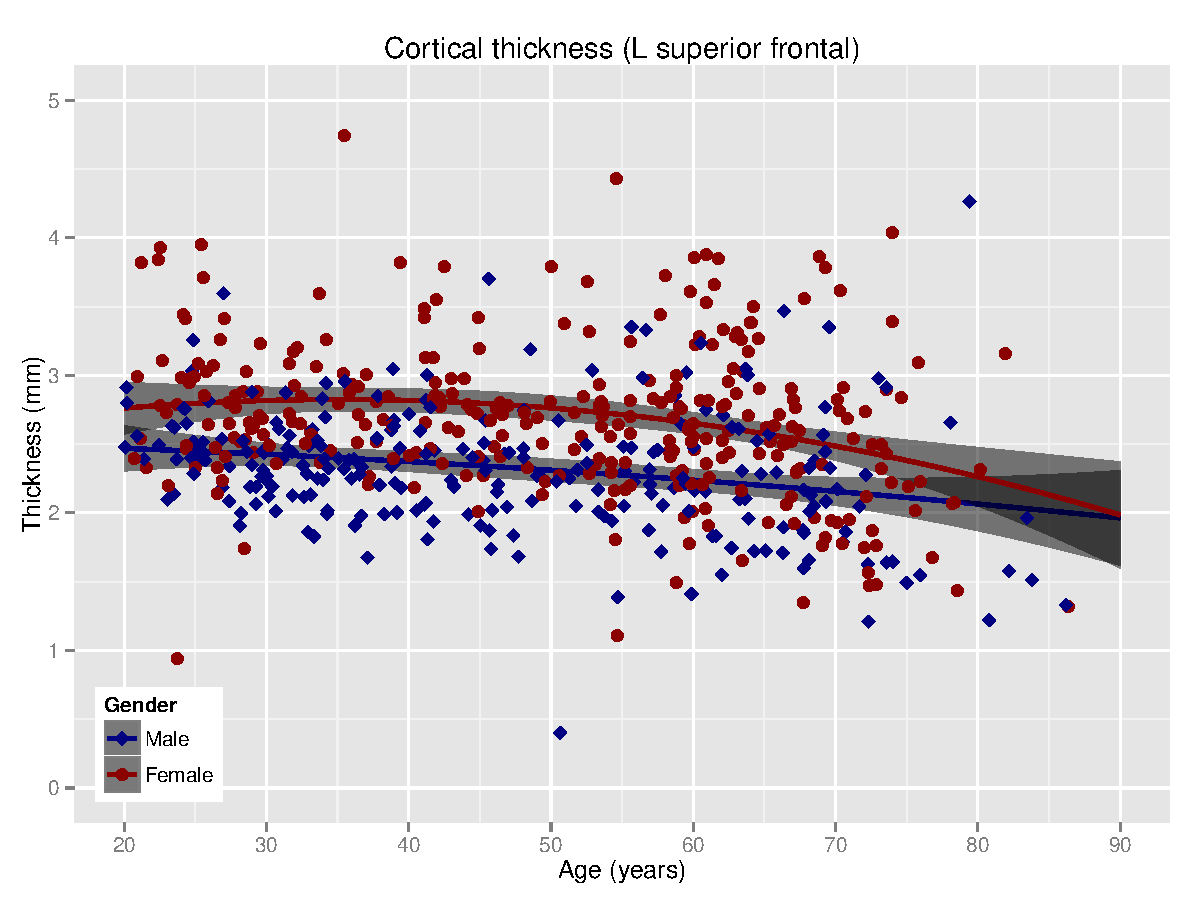
\includegraphics[width=57.5mm]{yylabel17_results.pdf} &
  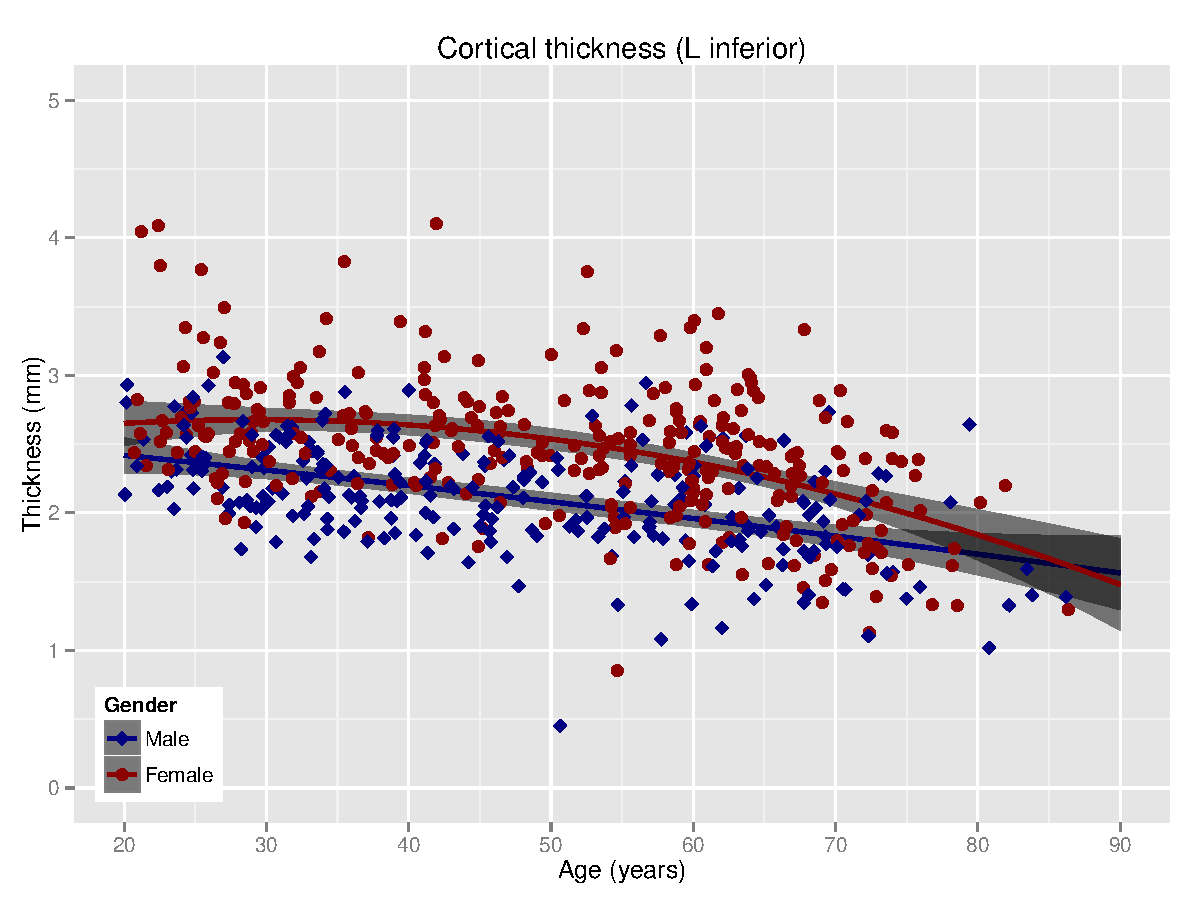
\includegraphics[width=57.5mm]{yylabel21_results.pdf} \\
  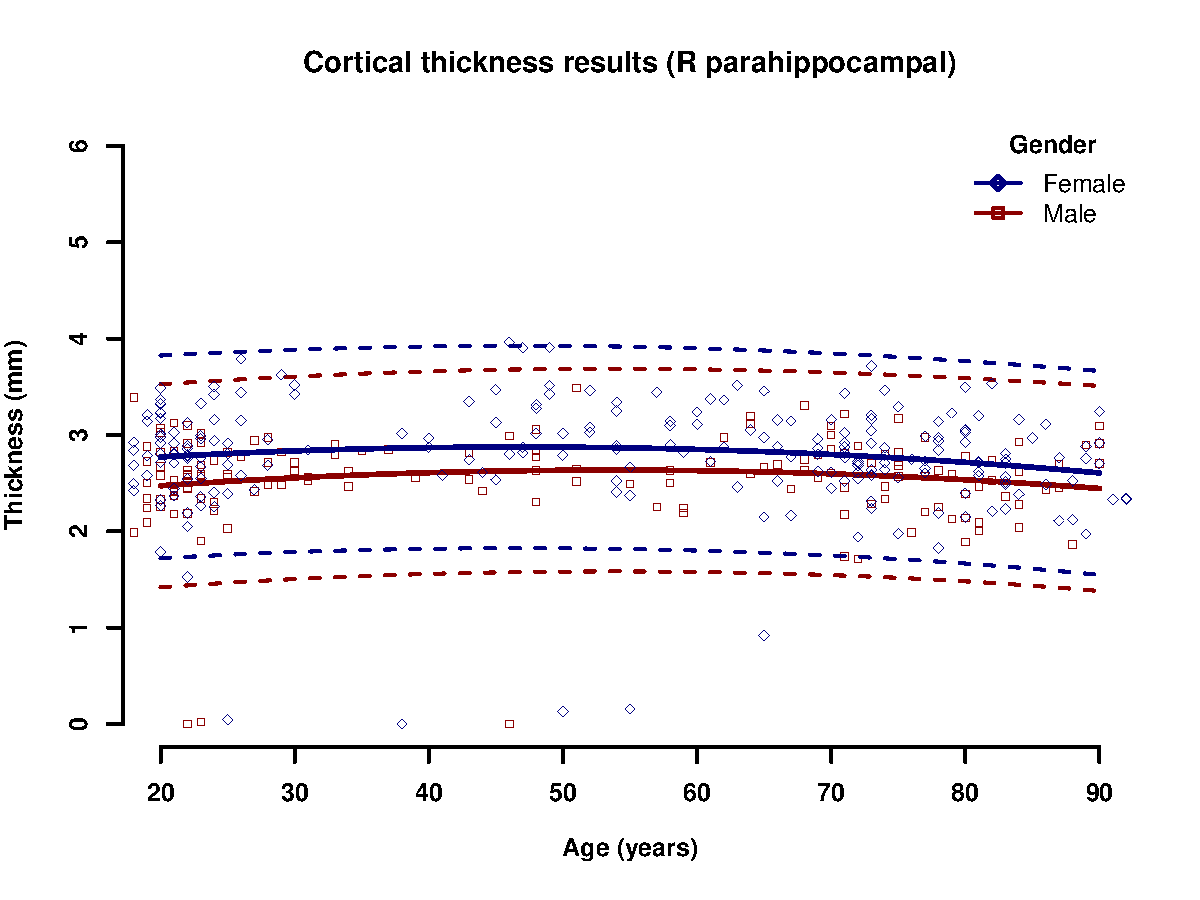
\includegraphics[width=57.5mm]{yylabel14_results.pdf} &
  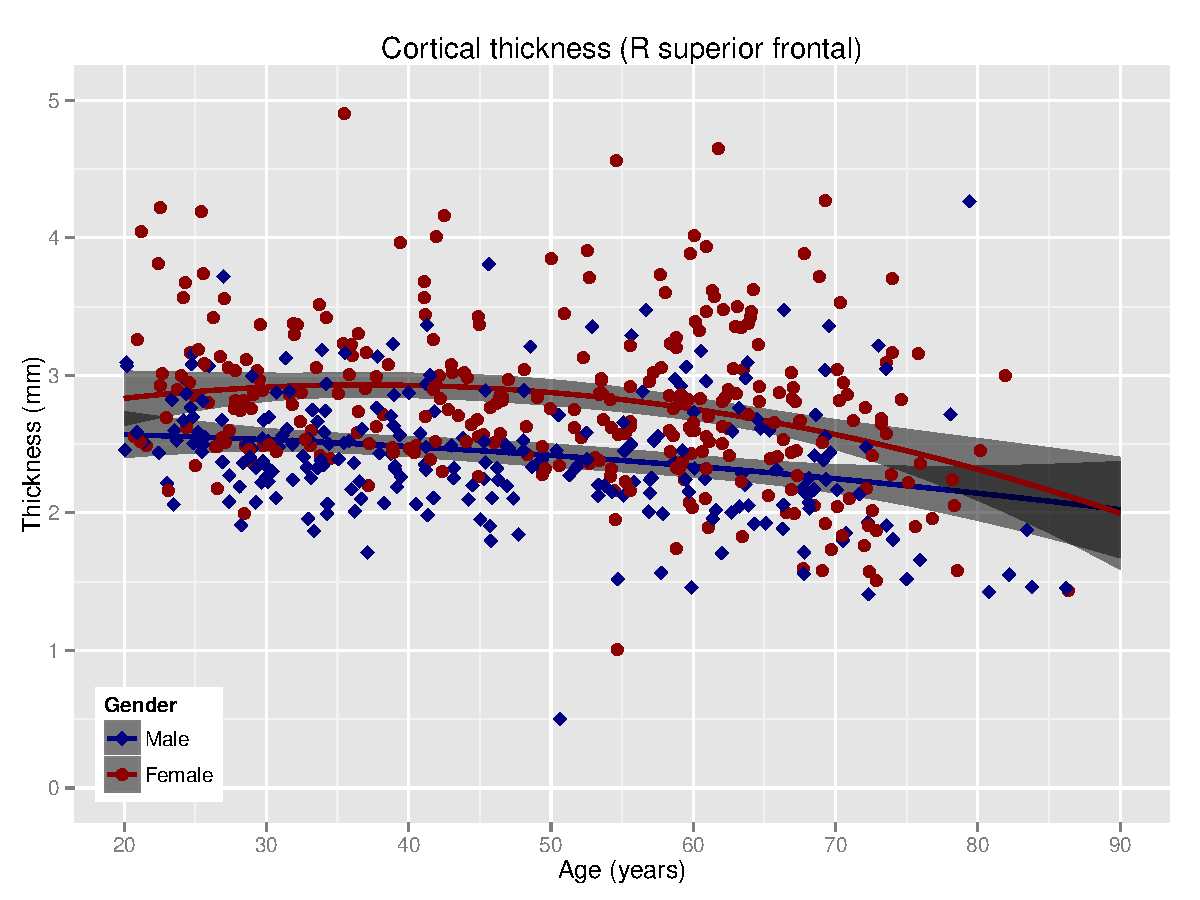
\includegraphics[width=57.5mm]{yylabel18_results.pdf} &
  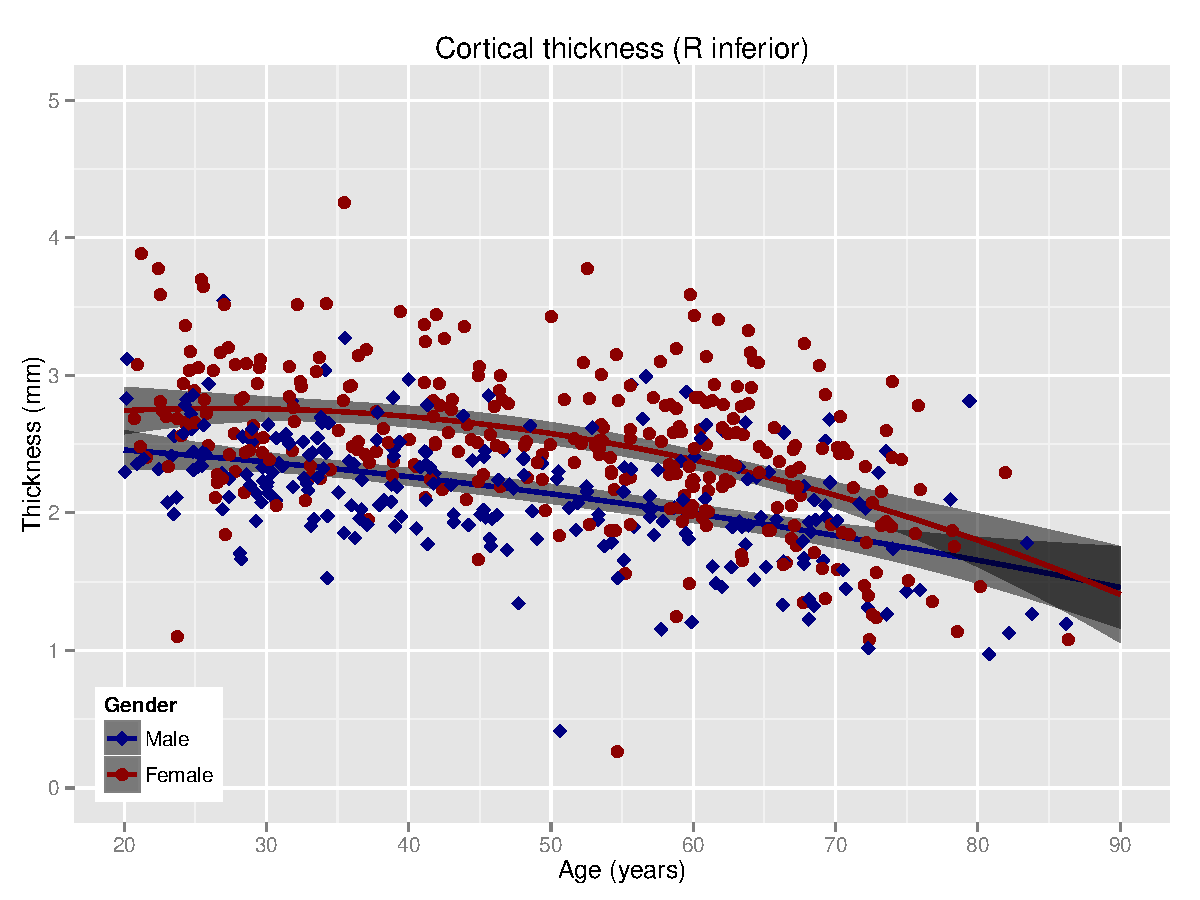
\includegraphics[width=57.5mm]{yylabel22_results.pdf} \\
  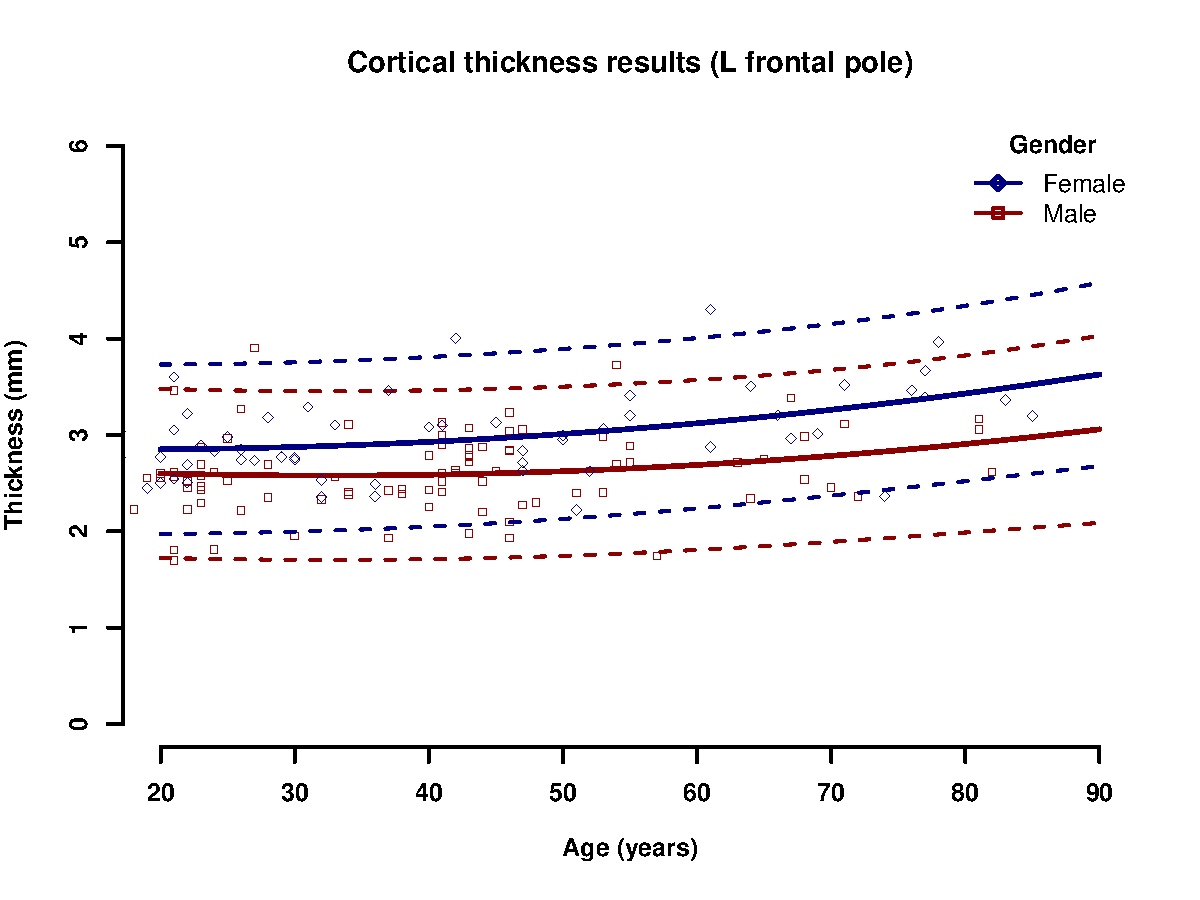
\includegraphics[width=57.5mm]{yylabel15_results.pdf} &
  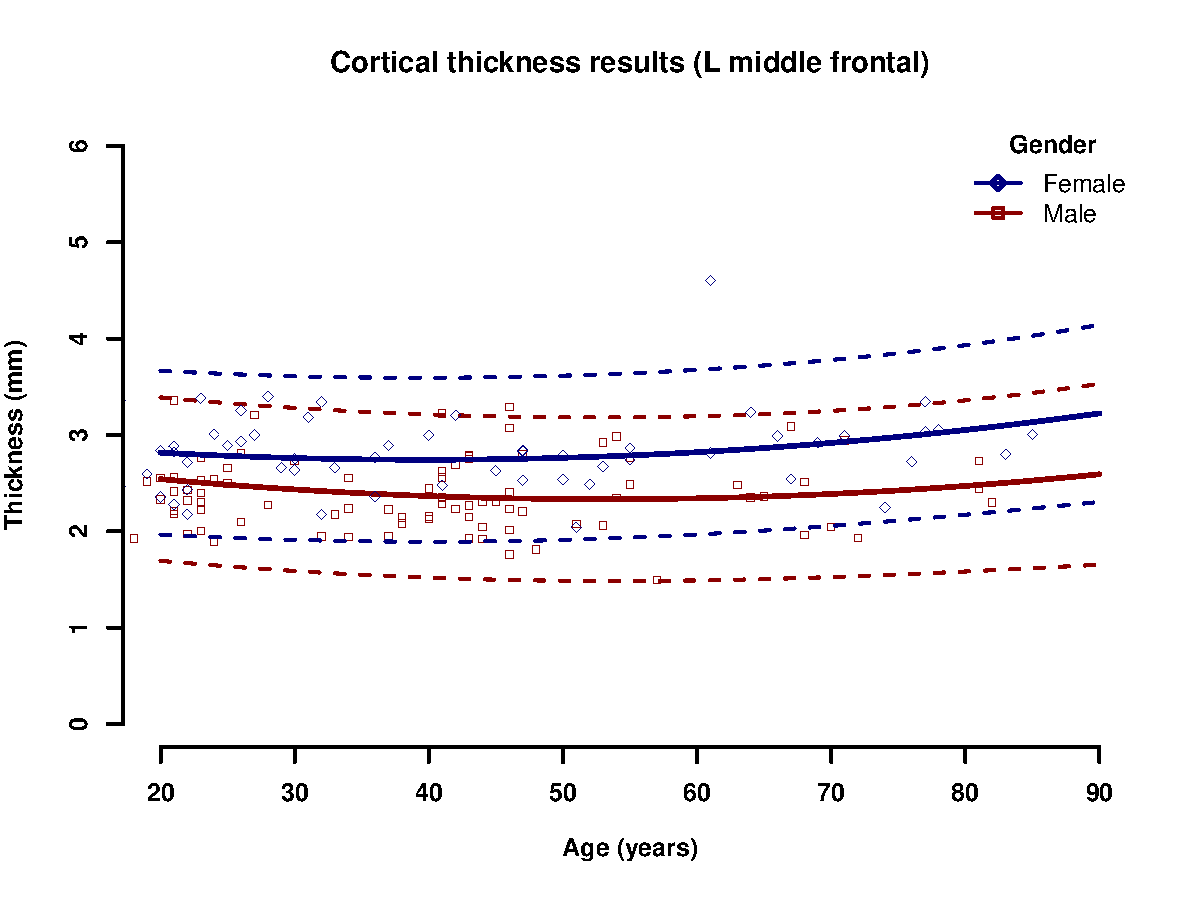
\includegraphics[width=57.5mm]{yylabel19_results.pdf} &
  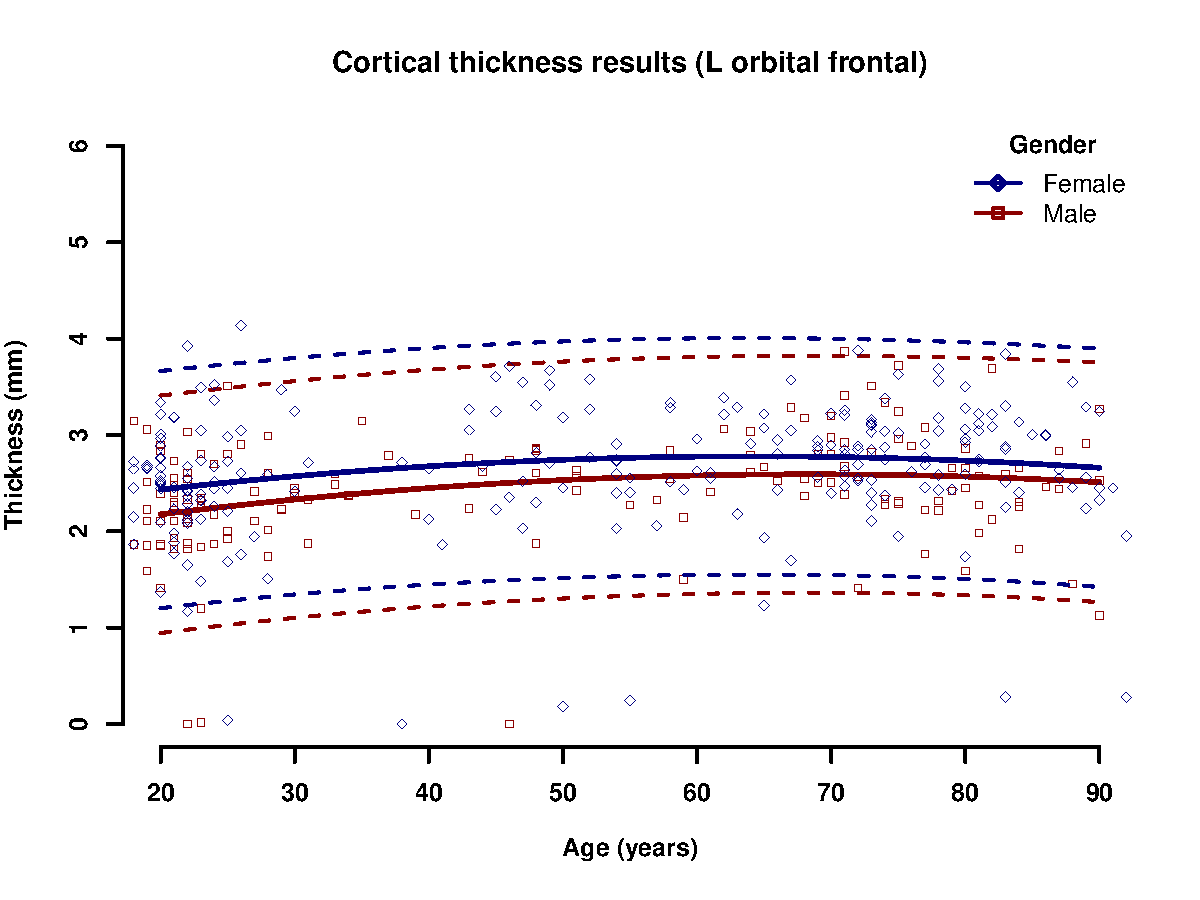
\includegraphics[width=57.5mm]{yylabel23_results.pdf} \\
  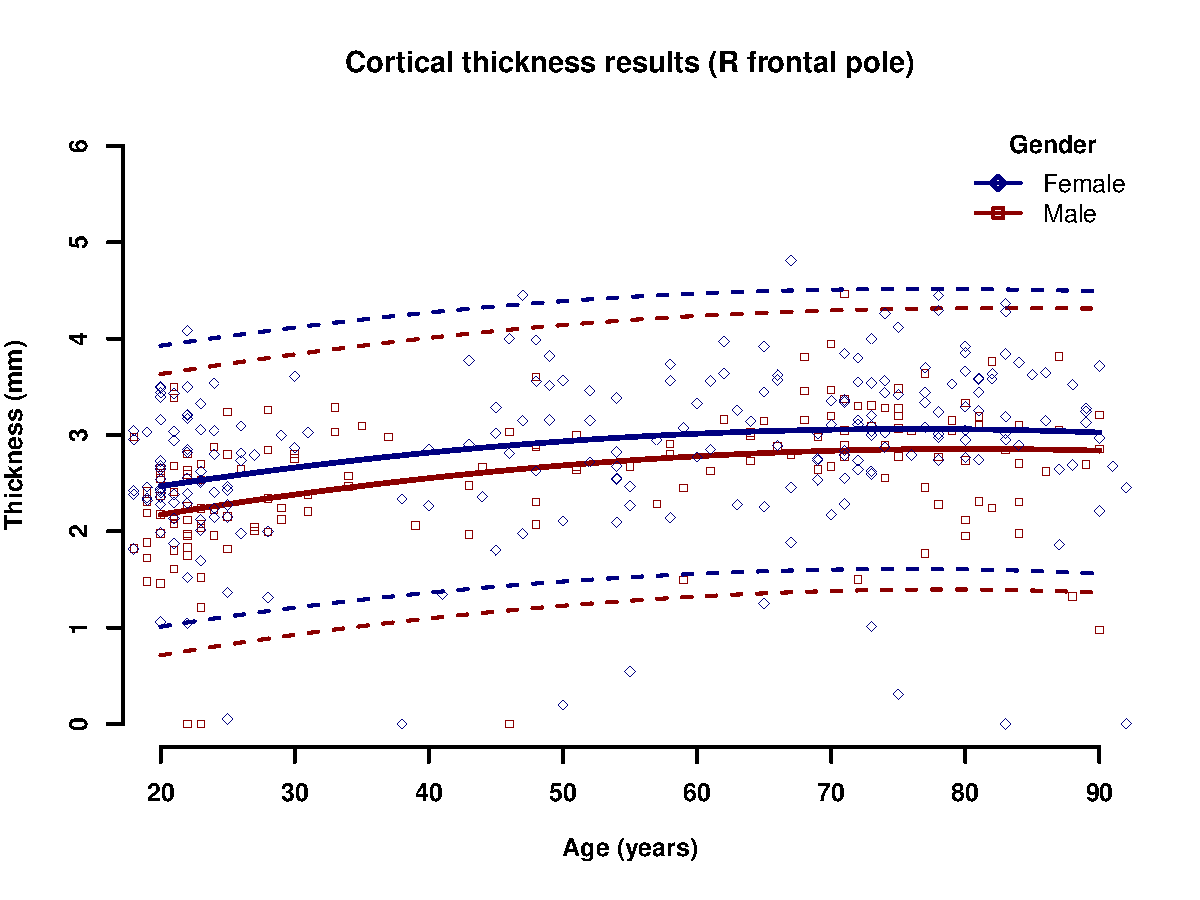
\includegraphics[width=57.5mm]{yylabel16_results.pdf} &
  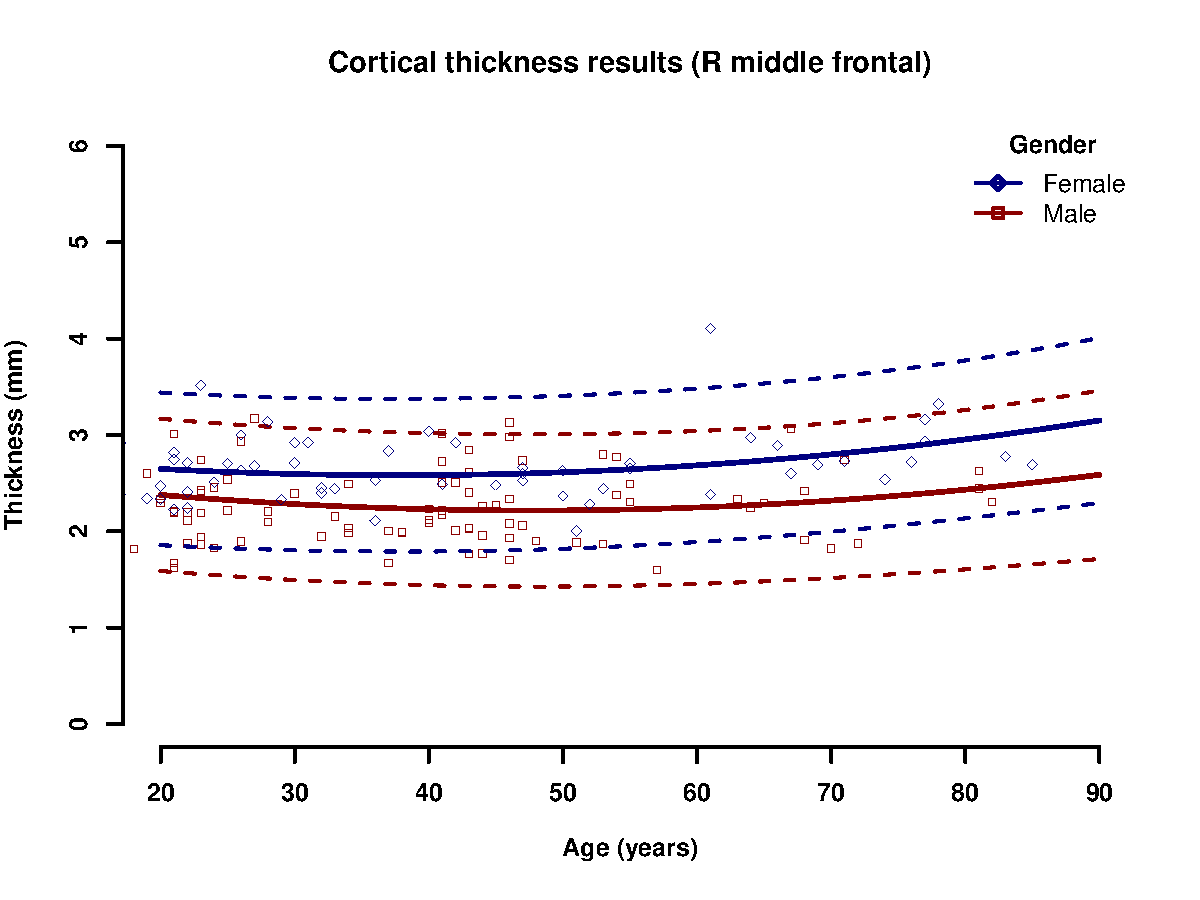
\includegraphics[width=57.5mm]{yylabel20_results.pdf} &
  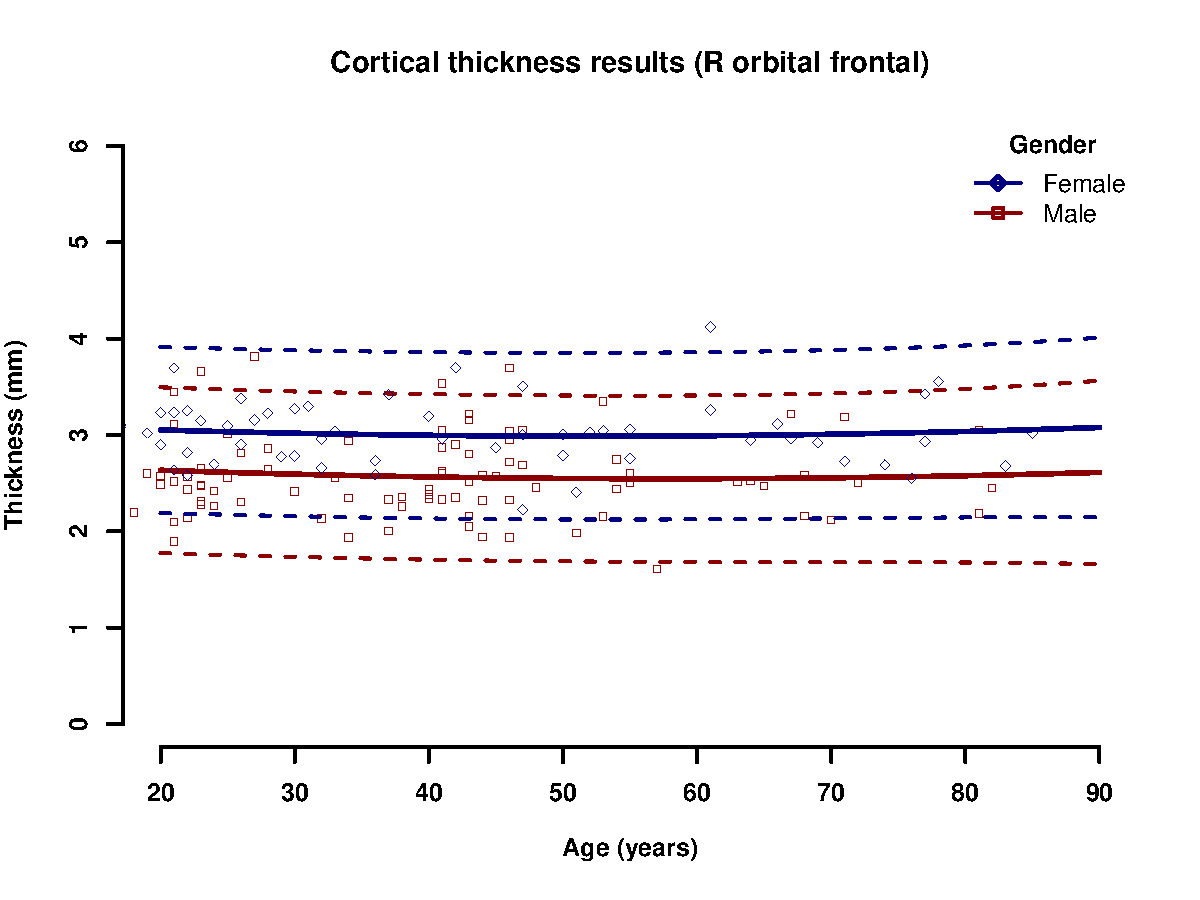
\includegraphics[width=57.5mm]{yylabel24_results.pdf} \\
  \end{tabular}
  \caption{Cortical thickness results (labels 13--24) from the IXI data set where
  each plot corresponds to one of the 32 cortical labels from the NIREP NA0 data set.  
  Thickness values have been normalized corresponding to the ratio of the individual 
  subject volume versus the total template volume.
  }
  \label{fig:nirep2}
\end{figure*}

\begin{figure*}
  \centering
  \begin{tabular}{cc}
  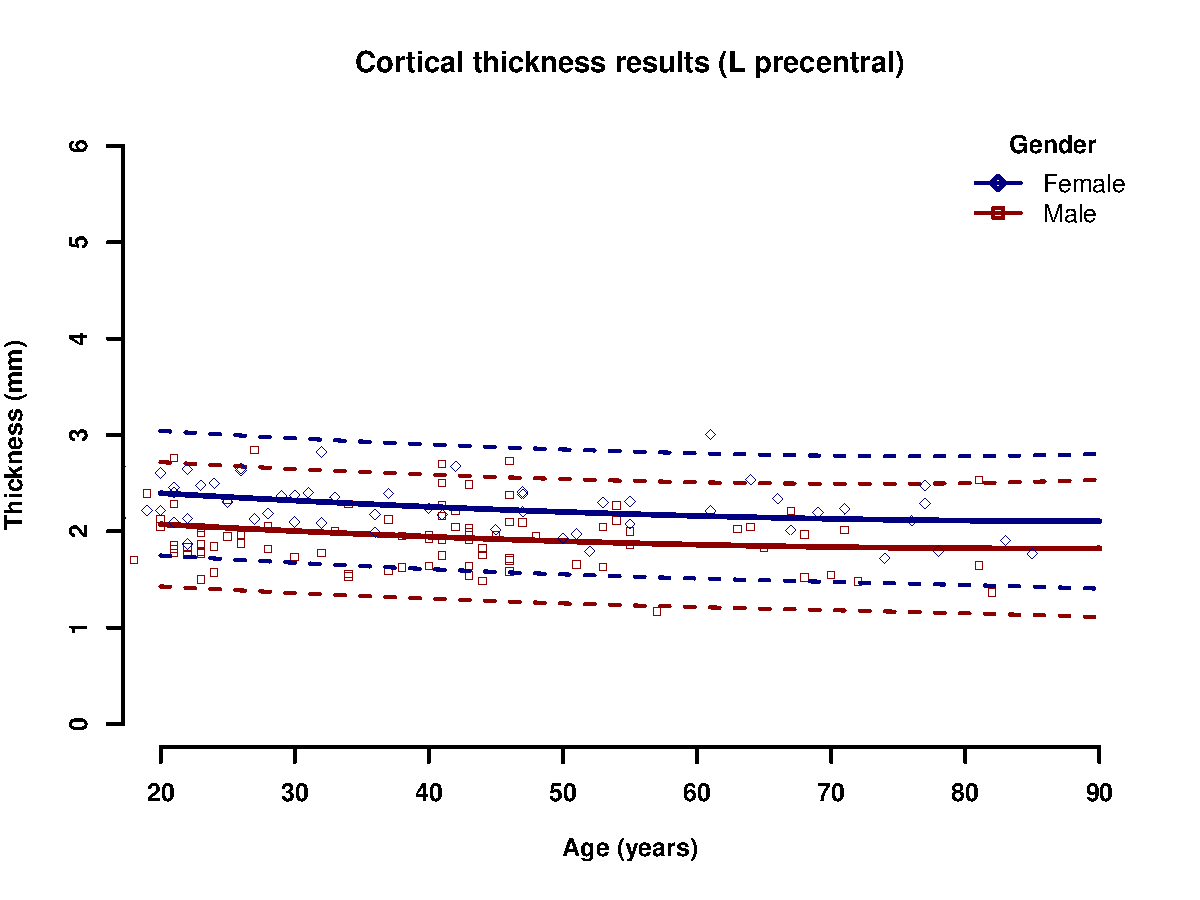
\includegraphics[width=57.5mm]{yylabel25_results.pdf} &
  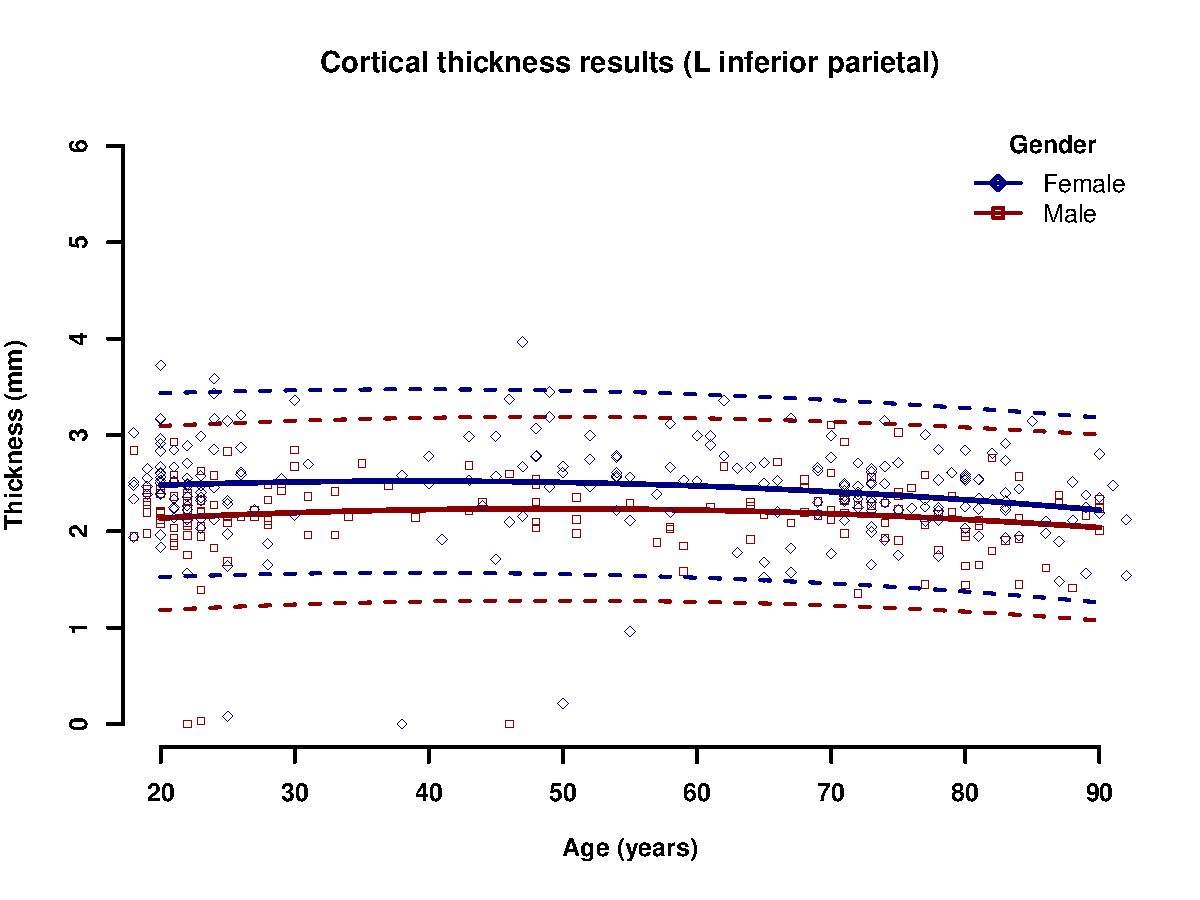
\includegraphics[width=57.5mm]{yylabel29_results.pdf} \\
  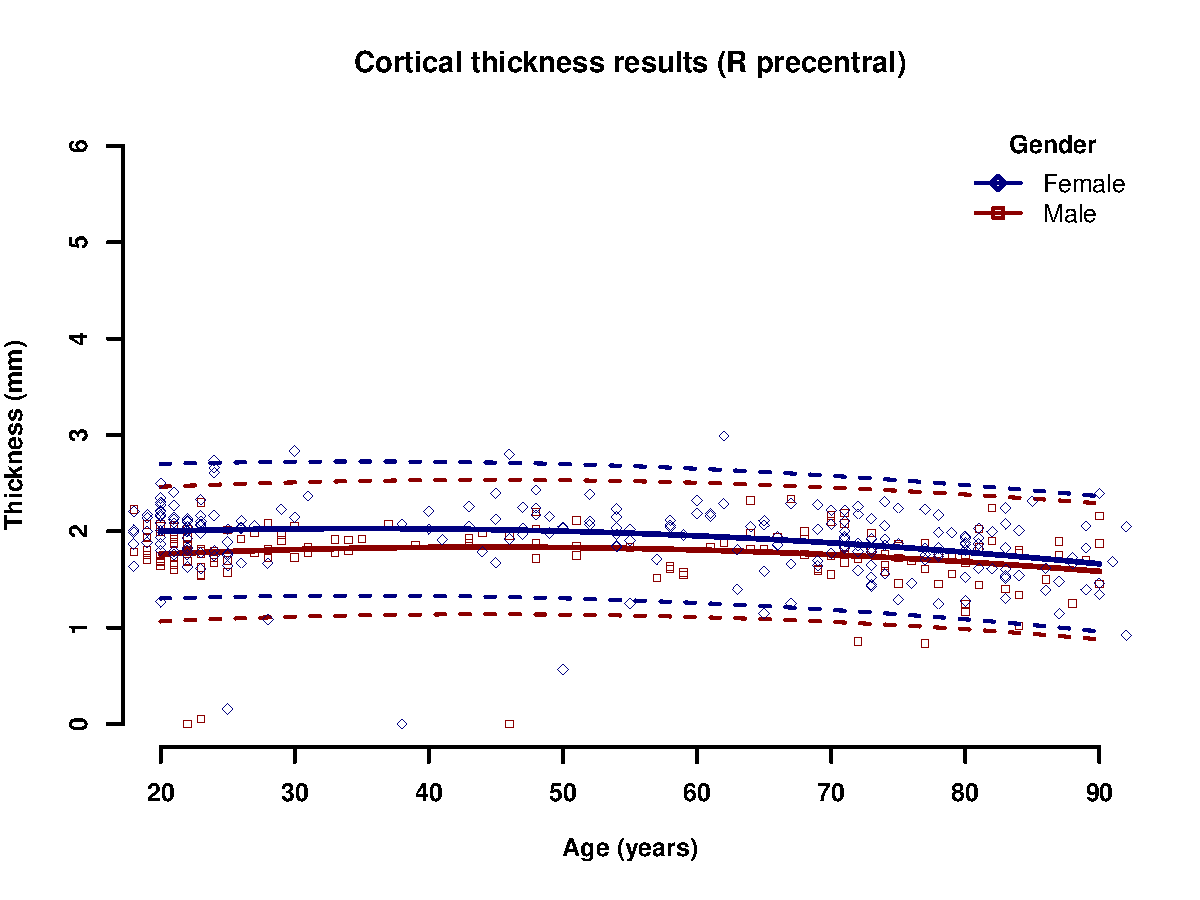
\includegraphics[width=57.5mm]{yylabel26_results.pdf} &
  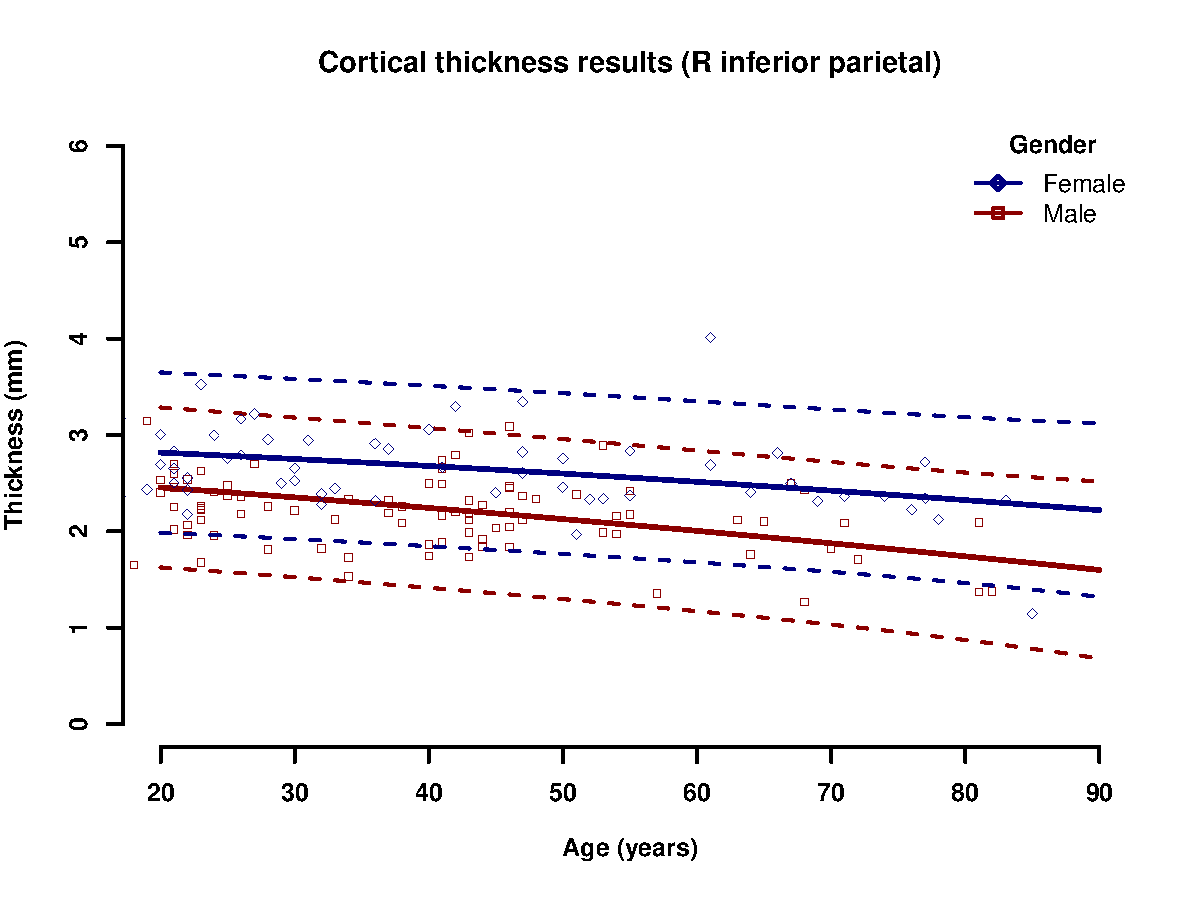
\includegraphics[width=57.5mm]{yylabel30_results.pdf} \\
  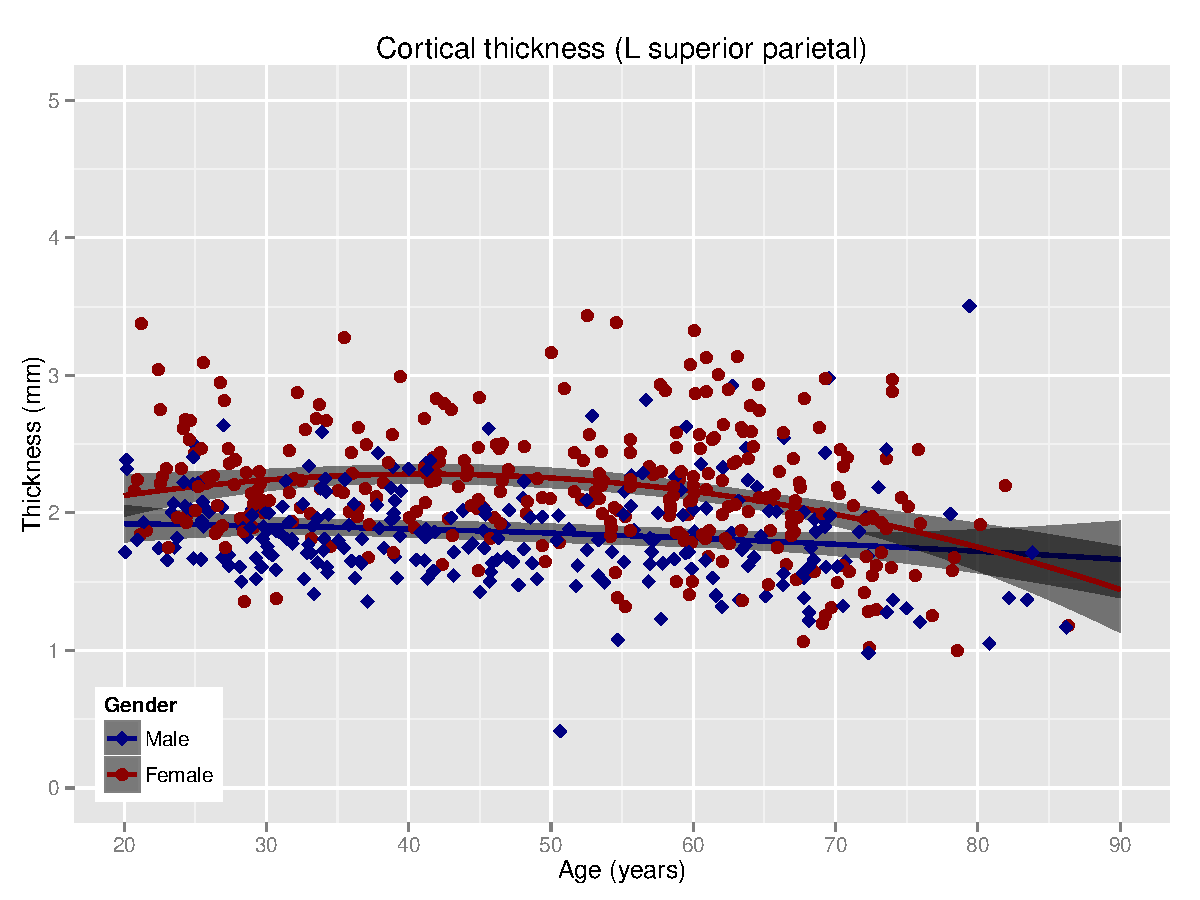
\includegraphics[width=57.5mm]{yylabel27_results.pdf} &
  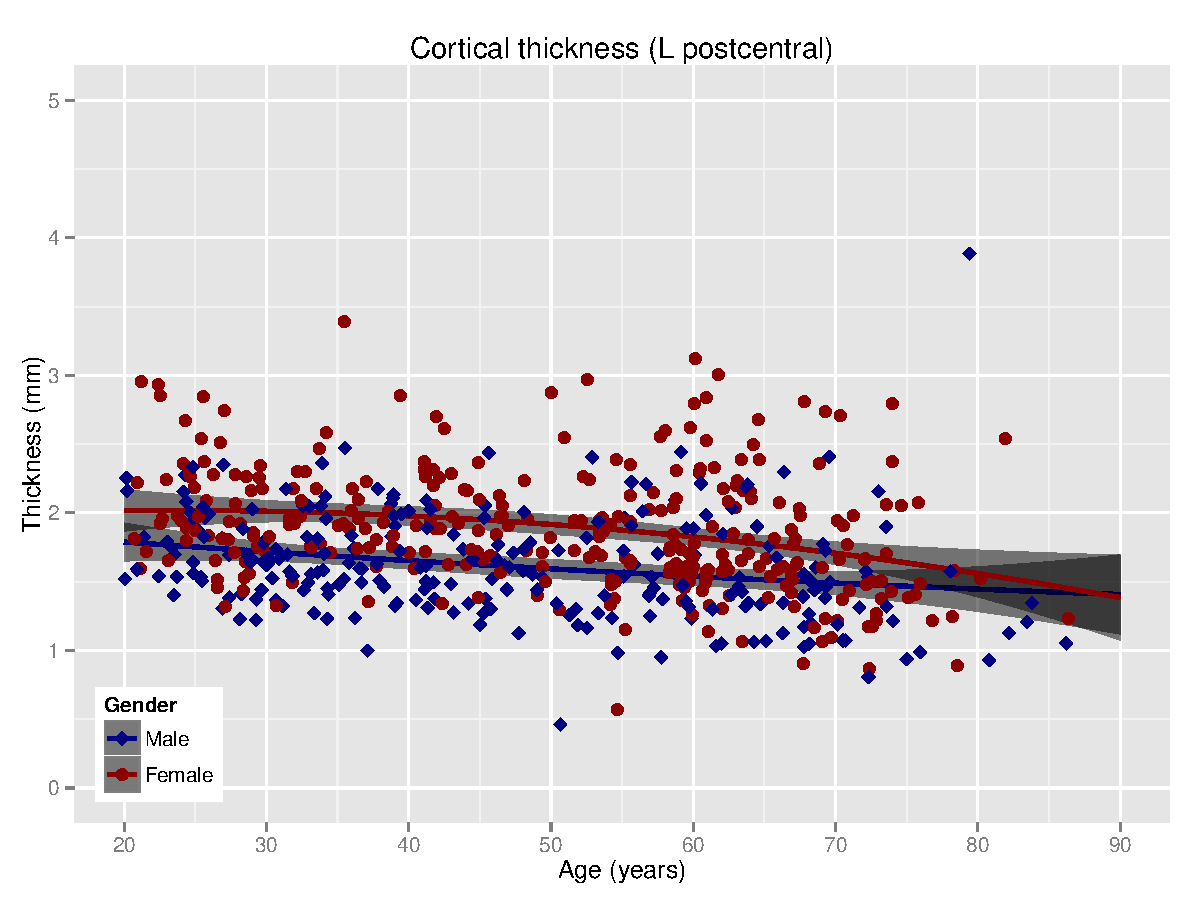
\includegraphics[width=57.5mm]{yylabel31_results.pdf} \\
  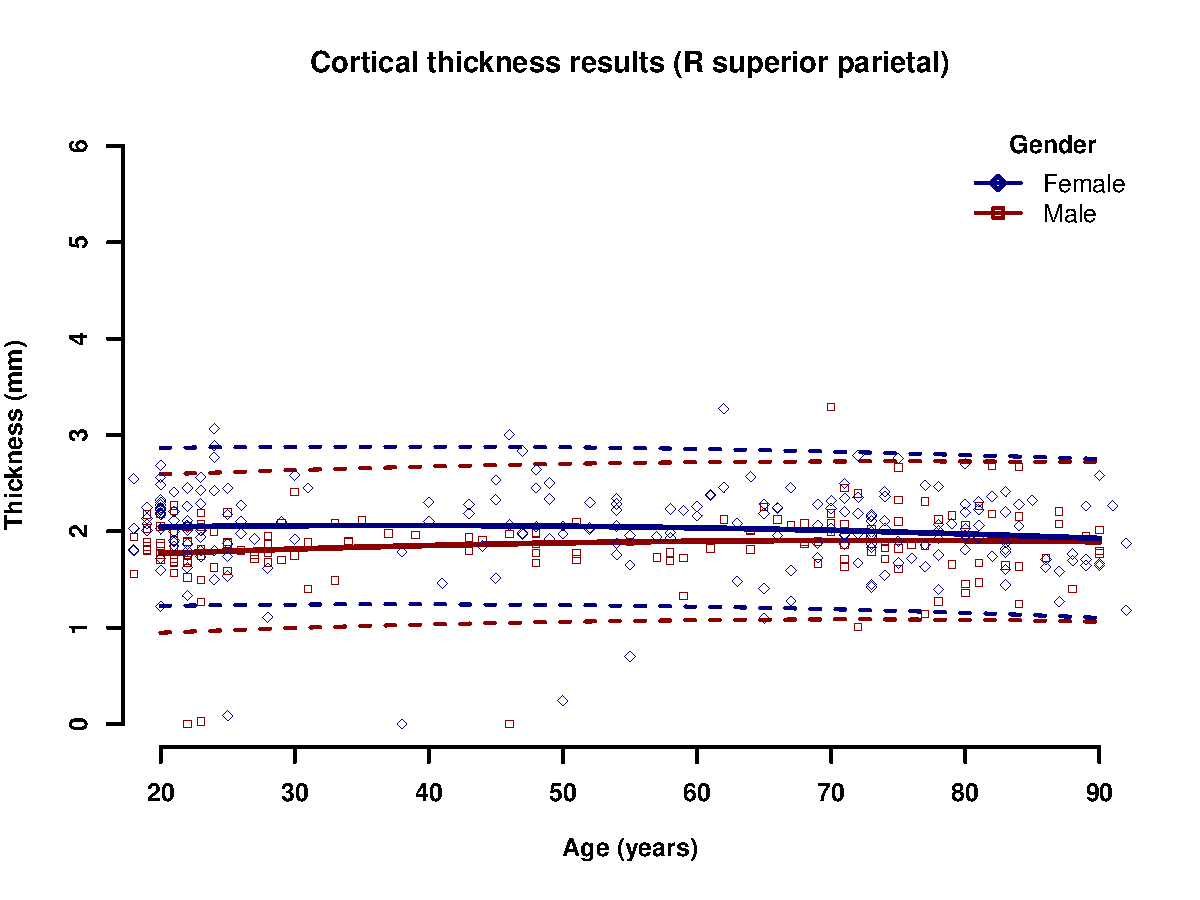
\includegraphics[width=57.5mm]{yylabel28_results.pdf} &
  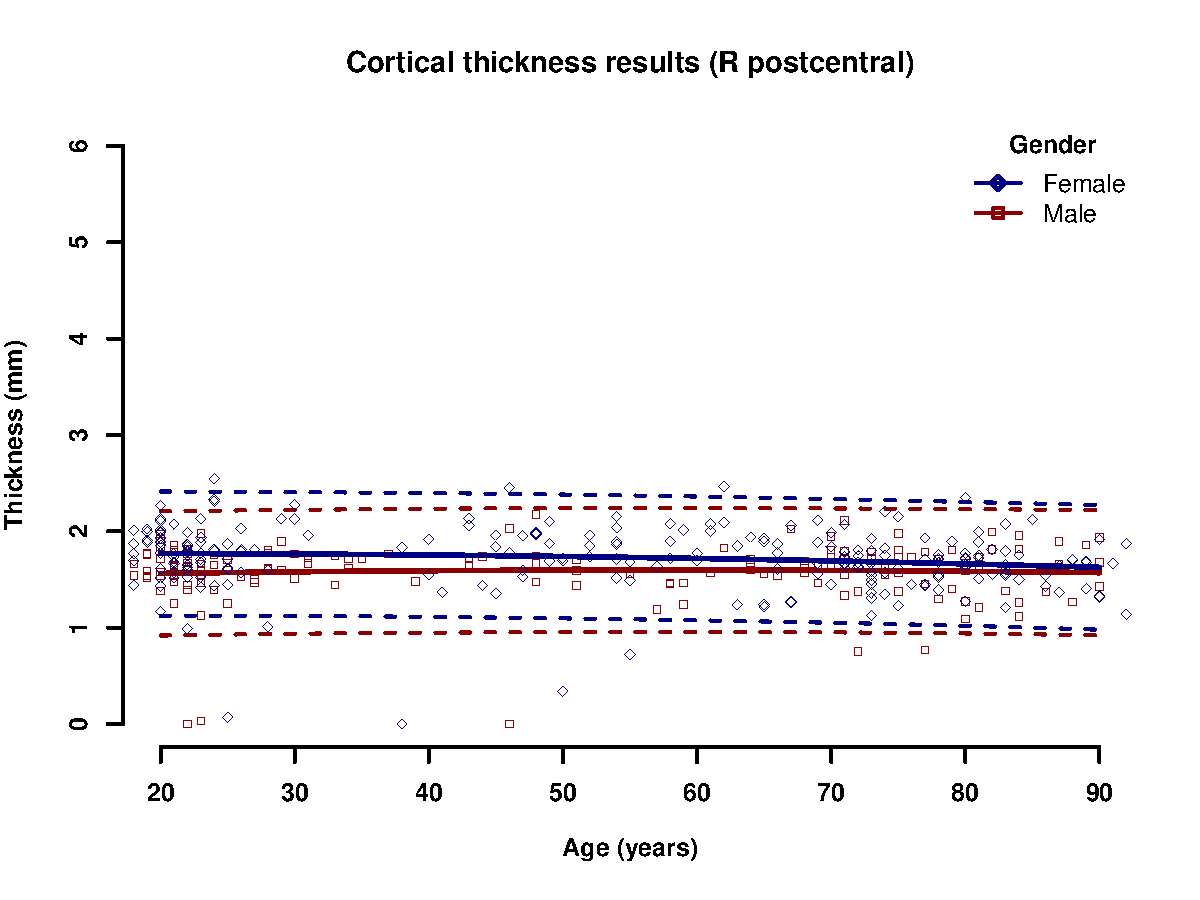
\includegraphics[width=57.5mm]{yylabel32_results.pdf} \\
  \end{tabular}
  \caption{Cortical thickness results (labels 25--32) from the IXI data set where
  each plot corresponds to one of the 32 cortical labels from the NIREP NA0 data set.  
  Thickness values have been normalized corresponding to the ratio of the individual 
  subject volume versus the total template volume.
  }
  \label{fig:nirep3}
\end{figure*}

